\documentclass[11pt]{article}
\usepackage[T1]{fontenc}
\usepackage[utf8]{inputenc}
\usepackage{lmodern}
\input{glyphtounicode}
\input{glyphtounicode-cmex}
\pdfgentounicode=1
\usepackage{tikz}
\usetikzlibrary{arrows.meta,positioning}
\usepackage[margin=1in]{geometry}
\usepackage{amsmath,amssymb,amsthm,mathtools}
\usepackage{microtype}
\usepackage{enumitem}
\usepackage{booktabs,array}
\usepackage{needspace}
\usepackage{xcolor}
\usepackage[hyphens]{url}
\usepackage{hyperref}
\hypersetup{colorlinks=true,linkcolor=blue!45!black,citecolor=blue!45!black,
  urlcolor=blue!45!black,
  pdftitle={A counterexample to Ryser's covering conjecture},pdfauthor={OpenAI}}
\urlstyle{same}
\setlength{\emergencystretch}{2em}
\setlist{itemsep=3pt,topsep=5pt}
\newtheorem{theorem}{Theorem}[section]
\newtheorem{lemma}[theorem]{Lemma}
\newtheorem{proposition}[theorem]{Proposition}
\newtheorem{corollary}[theorem]{Corollary}
\theoremstyle{remark}
\newtheorem{remark}[theorem]{Remark}
\newtheorem{definition}[theorem]{Definition}
\newcommand{\F}{\mathbb F}
\newcommand{\PP}{\mathbb P}
\newcommand{\R}{\mathbb R}
\newcommand{\N}{\mathbb N}
\newcommand{\E}{\mathbb E}
\DeclareMathOperator{\Var}{Var}
\DeclareMathOperator{\Cov}{Cov}
\DeclareMathOperator{\supp}{supp}
\title{A counterexample to Ryser's covering conjecture}
\author{OpenAI}
\date{September 23, 2026}

\begin{document}
\maketitle
\begin{abstract}
For every sufficiently large prime $s\equiv2\pmod3$ and every sufficiently
large odd integer $n$, with the threshold depending on $s$, we construct
an intersecting $(s^n+1)$-partite $(s^n+1)$-uniform hypergraph with covering
number $s^n+1$. This disproves Ryser's covering conjecture in its
intersecting case.
\end{abstract}

\section{Introduction}

A vertex cover of a finite hypergraph $H$ is a set of vertices meeting
every edge. Its covering number $\tau(H)$ is the minimum size of such a
set, and its matching number $\nu(H)$ is the maximum number of pairwise
disjoint edges. For an integer $r\ge2$, an $r$-partite $r$-uniform
hypergraph has disjoint vertex parts $V_1,\ldots,V_r$, with every edge
containing exactly one vertex from each part. Ryser's covering
conjecture asserts that every such hypergraph satisfies
\begin{equation}\label{eq:ryser}
 \tau(H)\le(r-1)\nu(H).
\end{equation}
A nonempty hypergraph is intersecting when every two distinct edges
meet; equivalently, its matching number is one. In this case the
conjecture asks for a cover of size at most $r-1$. The vertices of a
cover may lie in several different parts, which is the central
obstacle in constructing a counterexample.

For $r=2$, inequality~\eqref{eq:ryser} is K\H{o}nig's matching theorem.
An equivalent formulation appears in Henderson's 1971
thesis~\cite{Henderson1971}; Best and Wanless discuss the history of its
attribution to Ryser~\cite{BestWanless2018}. Aharoni proved the full
tripartite case~\cite{Aharoni2001}. In the intersecting case, the results
through rank four are due to Gy\'arf\'as, and the rank-five result to
Tuza, as recorded by Kir\'aly and T\'othm\'er\'esz~\cite{KiralyTothmeresz2017};
see also Tuza's early study of the covering conjecture~\cite{Tuza1983}.
Haxell and Scott proved $\tau(H)\le(r-\epsilon)\nu(H)$ for some
$\epsilon>0$ when $r=4$ or $5$, without assuming
intersection~\cite{HaxellScott2012}. White proved the particular
rank-four case $\nu(H)=2$, obtaining $\tau(H)\le6$~\cite{White2026}.\footnote{White
reports assistance from GPT-5.6 Sol and Claude in the Methods section
of his preprint.}
Under the additional assumption that any two distinct edges meet in
exactly one vertex, Franceti\'{c}, Herke, McKay, and Wanless established
the intersecting case through rank nine~\cite{FranceticHerkeMcKayWanless2017}.
Bishnoi, Das, Morris, and Szab\'o obtained bounds when every pair of
edges has a larger prescribed intersection~\cite{BDMS2021}.

Finite planes supply the classical equality examples. Delete a point
and all lines through it from a projective plane of order $q$. Partition
the remaining points according to the deleted line through them, and
take the remaining lines as hyperedges. The result is intersecting,
has $q+1$ parts and covering number $q$. Thus equality in the proposed
bound occurs whenever $r-1$ is a prime power. Work of Mansour, Song, and
Yuster~\cite{MansourSongYuster2009} and Aharoni, Bar\'{a}t, and
Wanless~\cite{AharoniBaratWanless2016} studies the structure and sparsity
of equality examples. Abu-Khazneh, Bar\'{a}t, Pokrovskiy, and
Szab\'{o} exploit the rigidity of minimum covers in a truncated plane
and add exceptional edges to obtain further equality
examples~\cite{AbuKhaznehBaratPokrovskiySzabo2019}. In that construction,
the number of parts and the covering number both increase by one.
Haxell and Scott combine affine planes with intersecting configurations
to obtain covering number at least $r-4$ for every sufficiently large
$r$, improved to $r-3$ when $r$ is even~\cite{HaxellScott2017}.

Our construction also starts from a finite plane and inserts exceptional
edges, but keeps one part for each ambient direction. It changes the
line labels within these parts to raise the covering number beyond
$q$. The following theorem gives the precise field orders for which
this can be done.

\begin{theorem}\label{thm:main}
There exists $s_0$ such that, for every prime $s\ge s_0$ with
$s\equiv2\pmod3$, there is an integer $n_0(s)\ge3$ with the following
property. For every odd integer $n\ge n_0(s)$, put $q=s^n$.
There is a finite intersecting $(q+1)$-partite $(q+1)$-uniform
hypergraph $H$ satisfying
\[
 \tau(H)=q+1.
\]
In particular, the intersecting case of~\eqref{eq:ryser} is false.
\end{theorem}

Every edge of a nonempty intersecting hypergraph is itself a cover,
so the assertion $\tau(H)\le q+1$ is automatic. The proof must construct
an intersecting hypergraph and exclude every cover of size at most $q$.
We first fix any sufficiently large eligible prime $s$, construct a
configuration in $\F_s^2$, and then take $n$ sufficiently large among
the odd integers. All subsequent thresholds may depend on that fixed
configuration. The result is asymptotic; the proof does not give a
numerical threshold.

A companion paper~\cite{OpenAI2026Balanced} proves a different theorem:
for every sufficiently large prime $q$, it constructs such a hypergraph
with exactly $q+1$ vertices in every part and with every vertex
nonisolated. Its construction modifies line partitions directly in the
prime plane. Here the field order is a proper odd power, and the proof
uses a small-field configuration with a nonlinear change of
coordinates. The two constructions give distinct ranges of ranks.
The only results imported from the companion are its three elementary
estimates in Appendix~A: the affine second-moment identity
(Lemma~A.1), bounded-drift concentration (Lemma~A.2), and the exposure
bound for independent trials (Lemma~A.3).

Lov\'asz proposed the stronger assertion that deleting $r-1$ vertices
can always reduce the matching number. Clow, Haxell, and Mohar
disproved that assertion at $r=3$~\cite{CHM2025}; Abiad, Garbe, Povill,
and Spiegel subsequently gave an infinite family at $r=3$ and
examples at $r=4$~\cite{AbiadGarbePovillSpiegel2025}. These examples
are consistent with~\eqref{eq:ryser}. They exclude a prescribed
matching-reduction procedure, whereas Theorem~\ref{thm:main}
violates the covering inequality itself.

\subsection*{Monochromatic tree covers}

An $r$-edge-coloring here assigns exactly one of $r$ colors to each edge.
A monochromatic tree cover is a family of monochromatic trees whose vertex
sets cover the graph; the trees may overlap, and singleton trees are allowed.
Gy\'arf\'as's conjecture asks whether $r-1$ such trees suffice for every
$r$-edge-colored complete graph; see \cite[Conjecture~1]{Milicevic2017}.
This is the covering formulation recorded after Theorem~2 in
\cite[Section~3]{ErdosGyarfasPyber1991}, not the distinct vertex-disjoint
tree-partition conjecture numbered Conjecture~2 there.

\begin{corollary}\label{cor:tree-cover}
Let $s_0$ and $n_0(s)$ be as in Theorem~\ref{thm:main}. For every prime
$s\ge s_0$ with $s\equiv2\pmod3$ and every odd integer $n\ge n_0(s)$,
put $r=s^n+1$. There is a finite simple complete graph with an
$r$-edge-coloring for which the minimum number of monochromatic trees
needed to cover its vertices is exactly $r$. The same minimum holds with
connected monochromatic subgraphs or maximal monochromatic components in
place of trees.
\end{corollary}

\begin{proof}
Take the hypergraph $H$ from Theorem~\ref{thm:main}, with parts
$V_1,\ldots,V_r$. For $e\in E(H)$, let $x_i(e)$ be the unique vertex in
$e\cap V_i$. Form the complete graph $K$ with vertex set $E(H)$. For each
pair of distinct hyperedges $e,f$, choose one index $i$ with
$x_i(e)=x_i(f)$ and color the edge $ef$ by $i$. Such an index exists
because $H$ is intersecting. Only one color is chosen even when the two
hyperedges meet in several parts.

Along a color-$i$ path, the value of $x_i$ is constant. Thus every connected
color-$i$ subgraph determines a vertex of $V_i$ belonging to every
hyperedge indexed by that subgraph. For a singleton, choose any color and
the corresponding vertex of its hyperedge. If $t$ connected monochromatic
subgraphs cover the vertices of $K$, the at most $t$ hypergraph vertices so
chosen meet every edge of $H$. Hence $t\ge\tau(H)=r$.

Conversely, fix a vertex of $K$. The $r$ monochromatic stars centered there,
one for each color and allowing singleton stars, cover all vertices of $K$.
They give a tree cover of size at most $r$. The lower bound applies to trees
and to maximal monochromatic components as well, and the stars can be
enlarged to maximal components. This proves all three stated minima.
\end{proof}

Thus Gy\'arf\'as's cover conjecture fails at these extension-field ranks.
The examples admit no cover by $r-1$ connected monochromatic subgraphs even
without a diameter restriction. They therefore also refute Mili\'cevi\'c's
bounded-diameter strengthening \cite[Conjecture~6]{Milicevic2017}, whose
diameter bound may depend on $r$, and the $\alpha=1$ case of the conjecture
of DeBiasio, Kamel, McCourt, and Sheats
\cite[Conjecture~2.8]{DeBiasioKamelMcCourtSheats2021}, whose diameter bound
depends only on the independence number $\alpha$. Indeed, $\alpha(K)=1$,
so the latter conjecture also demands a cover by at most $r-1$ such
subgraphs.

\subsection*{Proof strategy}

In the affine-plane model, the parts are indexed by the $q+1$ directions
in $\F_q^2$, and the vertices of a part are the $q$ lines of that
direction. A point $x$ defines an edge consisting of its incident line
in each direction. The edges of two points intersect at their join,
but a full parallel class always gives a cover of size $q$. We retain
many of these point edges and add exceptional edges whose labels are
changed in some directions. The construction has three tasks: preserve
intersection, restrict small covers of the retained point edges, and
make the exceptional edges too costly for those covers.

\paragraph{Restricting the ordinary cover.}
Delete a bounded number of translated shapes in each of $O(q)$
independent trials. The shapes are lines or curves that meet every
line in boundedly many points. Thus a shape has bounded intersection
with a line unless it is that line itself. Section~\ref{sec:linecover} proves that, under explicit
uniform survival assumptions, every cover of almost all surviving
points by at most $q$ lines contains almost a pencil. Here a pencil is
a family of lines through one projective point, including a parallel
class when that point is at infinity. Surviving points on each
nondeleted line then force every nondeleted member of this pencil
into the cover. To obtain the pencil statement over the required
extension fields, Section~\ref{sec:incidence} first proves an incidence
saving by the sum--product method of Bourgain, Katz, and
Tao~\cite{BKT2004}. Its constants are uniform over fields whose proper
subfields all have order at most $q^{1/3}$.

\paragraph{One configuration in two coordinates.}
In a fixed prime plane $\F_s^2$, remove one line in each finite nonzero
direction and call the remaining set $Y$. The change of coordinates
$f(x,y)=(x^3,y)$ is bijective when $s\equiv2\pmod3$. Original line
labels determine which ambient point edges must be deleted to
intersect the exceptional edges. The labels for altered directions
are instead read from the lines through $f(w)$, for $w\in Y$.
The map $f$ preserves the horizontal and vertical parallel classes;
this ensures intersection within the exceptional configuration.
Its nonlinear action on the other lines makes their images curves
with at most three intersections with any line. Applying the deletion
lemma in these new coordinates yields the crucial obstruction:
covering $f(Y)$ by $a$ lines and $b$ individual points with
$a+b/2\le s$ requires exactly one full parallel class and no point
resources. Section~\ref{sec:gadget} proves this statement together
with the ordinary-coordinate occupancy needed later.

\paragraph{Placing the configurations and spending the cover budget.}
Embed linearly transformed copies of $Y$ in $\F_q^2$ so that every
ambient direction is altered in one or two copies. Arbitrary translates
could create disjoint exceptional edges. We therefore sample a fixed
number of independent candidate translates for each copy.
Section~\ref{sec:selection} proves that one can choose compatible
representatives from these pools, using an independent-transversal
argument in the tradition of Haxell~\cite{Haxell1995,Haxell2001}.
Section~\ref{sec:placement} proves the deletion estimates for the
entire independent pool before making this selection. Keeping only
the selected deletions restores ordinary points, so the needed
estimates transfer by deterministic inclusion.

Section~\ref{sec:hypergraph} gives the labels of every edge, proves
intersection, and excludes a cover of size at most $q$. After the
ordinary edges force a pencil, its center determines the remaining
argument. At infinity, the uncovered exceptional configurations
require more vertices than the missing parallel lines release.
Inside an embedded configuration, the remaining budget would cover
$f(Y)$ by at most $s$ lines including two nonparallel axis lines.
Outside every configuration, each deleted pencil line supplies five
uncovered exceptional edges, while every additional vertex covers at
most five. In all three cases the available budget is too small.

\paragraph{Conventions.}
A direction is a one-dimensional linear subspace of $\F_q^2$; as a subspace
it includes zero. The projective completion adds one point at infinity per
direction. A pencil consists of the affine lines through a projective point:
it has $q+1$ members for a finite center and $q$ members for a center at
infinity. Thus concurrence always includes parallel lines.
For a positive integer $j$, write $(a)_j=a(a-1)\cdots(a-j+1)$.
All asymptotic constants may depend on the parameters explicitly held fixed.
An event holds with high probability if its probability tends to one along
the specified sequence of fields. The small field is fixed before the
ambient field tends to infinity.

\section{A uniform incidence bound}\label{sec:incidence}

For a set $P$ of points and a set $\mathcal L$ of lines in
$\PP^2(\F_q)$, write
\begin{equation}\label{eq:inc-definition}
 I(P,\mathcal L)
 =\bigl|\{(p,\ell)\in P\times\mathcal L:p\in\ell\}\bigr|.
\end{equation}
Our aim is a power saving with constants independent of the field and
its characteristic. In Section~\ref{sec:linecover}, this estimate will
control intersections of a proposed line cover when no projective point
lies on many of its lines. This is the incidence input to the conclusion
that a small cover must contain almost a full pencil.

\begin{theorem}[Uniform incidence saving]\label{thm:incidence}
There exist absolute constants $\kappa\in(0,1/10)$ and $Q$ with the following
property. Suppose that $q\ge Q$ is a prime power and every proper subfield
of $\F_q$ has order at most $q^{1/3}$. If $P$ and $\mathcal L$ are sets of
projective points and projective lines over $\F_q$ satisfying
\begin{equation}\label{eq:inc-theorem-sizes}
 |P|,|\mathcal L|\le q^{1+\kappa},
\end{equation}
then
\begin{equation}\label{eq:inc-theorem-bound}
 I(P,\mathcal L)\le q^{3/2-\kappa}.
\end{equation}
\end{theorem}

The proof follows the incidence and sum--product strategy of
Bourgain, Katz, and Tao~\cite[Sections 3--4 and 6]{BKT2004}. Its geometric
step turns an incidence configuration with too many incidences into a
dense set of pairs whose differences and quotients range over small
sets. A graph argument then extracts one subset with both a small
difference set and a small quotient set. Finally, scalar coverings show
that such a subset cannot have size near the square root of the field
order under the proper-subfield hypothesis.

We develop the two algebraic ingredients first, then return to the
incidence configuration. The proofs include the simultaneous extraction
of additive and multiplicative control and the bounds on scalar
expressions that make the argument uniform over fields of nonprime
order.

\subsection{Finite-set estimates}

The first task is to pass from control of differences and quotients
along the edges of a dense bipartite graph to control on all pairs in
one subset. We begin with the sumset estimates needed to use the
resulting additive control.

For subsets of an abelian group, $X+Y$ and $X-Y$ denote the usual sumset
and difference set. For a nonnegative integer $j$, the notation $jY$
in this subsection means a sum of $j$ copies of $Y$, with $0Y=\{0\}$.
Later, a field element multiplying a set will always mean field scaling;
we will specify explicitly when an integer denotes an iterated sumset.

The first two estimates below are Ruzsa's triangle inequality and
covering lemma; the maximal-translates proof of the latter appears in
\cite[p.~324]{Ruzsa1999}. The multiple-sum bound is a Pl\"unnecke--Ruzsa
estimate, for which we use Petridis's minimizing-subset
proof~\cite[Proposition 2.1 and Section 3]{Petridis2012}.

\begin{lemma}[Triangle, covering, and multiple-sum estimates]
\label{inc-sumset-estimates}
Let the sets below be finite subsets of an abelian group.
\begin{enumerate}
\item If $Z$ is nonempty, then
\begin{equation}\label{eq:inc-triangle}
 |X-Y|\,|Z|\le |X-Z|\,|Z-Y|.
\end{equation}
\item If $Y$ is nonempty and $|X-Y|\le M|Y|$, then $X$ is contained in
the union of at most $M$ translates of $Y-Y$.
\item If $Y$ is nonempty and $|Y-Y|\le M|Y|$, then, for all nonnegative
integers $u,v$,
\begin{equation}\label{eq:inc-multiple-sums}
 |uY-vY|\le M^{u+v}|Y|.
\end{equation}
\end{enumerate}
\end{lemma}

\begin{proof}
For the triangle inequality, choose one representation $d=x_d-y_d$
for each $d\in X-Y$. The map
\[
 (d,z)\longmapsto (x_d-z,z-y_d)
\]
from $(X-Y)\times Z$ into $(X-Z)\times(Z-Y)$ is injective: summing the
two coordinates recovers $d$, after which the chosen representation
recovers $z$. This proves~\eqref{eq:inc-triangle}.

For the covering statement, take a maximal set $T\subseteq X$ for
which the translates $t-Y$, $t\in T$, are pairwise disjoint. Their union
is contained in $X-Y$, so $|T|\le M$. Maximality implies that for every
$x\in X$ some $x-Y$ intersects $t-Y$ with $t\in T$, whence
$x\in t+(Y-Y)$.

For the multiple-sum bound, the minimizing-subset argument of
Petridis~\cite{Petridis2012} lets us iterate a one-step growth estimate.
Put $Q_0=-Y$ and choose a nonempty
$W\subseteq Y$ minimizing
\[
 \mu=\frac{|W+Q_0|}{|W|}.
\]
Then $\mu\le M$, and every $W'\subseteq W$, including the empty set,
satisfies $|W'+Q_0|\ge\mu|W'|$. We claim that for every finite set $E_0$,
\begin{equation}\label{eq:inc-petridis-growth}
 |W+Q_0+E_0|\le\mu|W+E_0|.
\end{equation}
The assertion is immediate if $E_0$ is empty. Otherwise order its
elements as $e_1,\ldots,e_k$. When the translate $W+e_i$ is added to
the preceding translates, let
\[
 W_i'=\{w\in W:w+e_i\in\bigcup_{j<i}(W+e_j)\}.
\]
It contributes exactly $|W|-|W_i'|$ new elements. Moreover,
$W_i'+Q_0+e_i$ is contained in the union of the preceding enlarged
translates $W+Q_0+e_j$. Thus the contribution of $W+Q_0+e_i$ is at most
\[
 |W+Q_0|-|W_i'+Q_0|
 \le\mu\bigl(|W|-|W_i'|\bigr).
\]
Summing proves~\eqref{eq:inc-petridis-growth}. Iterating this estimate
gives $|W+jQ_0|\le\mu^j|W|$ for every nonnegative integer $j$.
We now remove the auxiliary set $W$ by applying
\eqref{eq:inc-triangle} to $uQ_0,vQ_0$ with intermediate set $-W$:
\[
 |uQ_0-vQ_0|\,|W|
 \le |W+uQ_0|\,|W+vQ_0|
 \le\mu^{u+v}|W|^2.
\]
Negation preserves cardinality, so $|uQ_0-vQ_0|=|uY-vY|$. Since
$|W|\le|Y|$ and $\mu\le M$, this is~\eqref{eq:inc-multiple-sums}.
\end{proof}

We next carry out the extraction from a dense graph. The argument uses
the common-neighborhood method in Gowers's quantitative refinement
\cite[Section 4, Lemma 11 and Proposition 12]{Gowers1998} of the
Balog--Szemer\'edi theorem~\cite{BalogSzemeredi1994}; see also
\cite[Section 5, Lemmas 5.1--5.2]{FoxSudakov2011}. The point is to use the same walks
for both additive and multiplicative edge labels. We can therefore
obtain both bounds on one subset, which is what the subsequent
subfield argument requires. In the geometric application, the edge
labels will come from the four pencils through four chosen points.

\begin{lemma}[Simultaneous difference and quotient extraction]
\label{inc-simultaneous-extraction}
Let $F$ be a field, let $A,B\subseteq F^*$ be finite, and let
$G\subseteq A\times B$. Define
\[
 D=\{a-b:(a,b)\in G\},\qquad
 J=\{a/b:(a,b)\in G\}.
\]
Suppose that, for real numbers $n>0$ and $V\ge2$,
\begin{equation}\label{eq:inc-graph-hypotheses}
 |A|,|B|,|D|,|J|\le Vn,
 \qquad |G|\ge n^2/V.
\end{equation}
Then there is $S\subseteq A$ such that
\begin{equation}\label{eq:inc-extracted-size}
 \frac{3n}{8V^2}\le |S|\le Vn
\end{equation}
and
\begin{equation}\label{eq:inc-extracted-expansion}
 |S-S|,|S/S|\le 2^{20}V^{22}n.
\end{equation}
Here $S/S=\{a/a':a,a'\in S\}$.
\end{lemma}

\begin{proof}
We first find a large set of vertices such that every ordered pair
is joined by many walks of length four. Counting the possible edge
labels of these walks will then bound both differences and quotients
of the endpoints.

Regard $G$ as a bipartite graph, and put
$\tau=(512V^8)^{-1}$. Call an ordered pair $(a,a_2)\in A^2$ bad if
it has fewer than $\tau n$ common neighbors in $B$. To find a
neighborhood with few bad pairs, first note that vertices of $B$
with fewer than $n/(2V^2)$ neighbors account for at most
$|B|n/(2V^2)\le n^2/(2V)$ edges. Since every vertex of $B$ has at
most $Vn$ neighbors, the set of vertices with at least $n/(2V^2)$
neighbors has size at least $n/(2V^2)$.

Summed over all $b\in B$, the number of bad ordered pairs in the
neighborhood of $b$ is at most
\[
 |A|^2\tau n\le V^2\tau n^3.
\]
Averaging over the large neighborhoods just identified, one obtains
a neighborhood $A_0$ of size at least $n/(2V^2)$ in which the number
of bad ordered pairs is at most
\[
 2V^4\tau n^2=\frac{n^2}{256V^4}
 \le \frac{|A_0|^2}{64}
 \le \frac{|A_0|^2}{16}.
\]
Let $S$ consist of those $a\in A_0$ having at most $|A_0|/4$ bad
partners in $A_0$. At most $|A_0|/4$ elements are discarded, so
$|S|\ge3|A_0|/4$, proving~\eqref{eq:inc-extracted-size}.

The choice of $S$ ensures that, for every $a,a'\in S$, at least
$|A_0|/2$ elements $a_2\in A_0$ form nonbad pairs with both endpoints.
Each such $a_2$ gives at least $(\tau n)^2$
ordered walks
\[
 a,b_1,a_2,b_2,a'
\]
whose four edges belong to $G$. Repeated vertices are allowed.
Consequently each ordered endpoint pair in $S^2$ has at least
\begin{equation}\label{eq:inc-walk-count}
 \frac{|A_0|}{2}(\tau n)^2
 \ge\frac{n^3}{2^{20}V^{18}}
\end{equation}
such walks. This lower bound now converts the limited number of edge
labels into a bound on endpoint differences.

For one of these walks, write its edge differences, always taking
the $A$ coordinate minus the $B$ coordinate, as
\[
 d_1=a-b_1,\quad d_2=a_2-b_1,\quad
 d_3=a_2-b_2,\quad d_4=a'-b_2.
\]
They satisfy $a-a'=d_1-d_2+d_3-d_4$. For a fixed endpoint pair,
the four differences determine the walk uniquely: starting from $a$,
one recovers successively $b_1,a_2,b_2,a'$. Choose one ordered
endpoint pair for each element of $S-S$. The resulting collections
of difference quadruples are disjoint for different differences,
because their alternating sums differ. Counting in $D^4$ and using
\eqref{eq:inc-walk-count} gives
\[
 |S-S|\le
 \frac{|D|^4}{n^3/(2^{20}V^{18})}
 \le 2^{20}V^{22}n.
\]

The same walks give the quotient bound on the same set $S$. Put
\[
 j_1=a/b_1,\quad j_2=a_2/b_1,\quad
 j_3=a_2/b_2,\quad j_4=a'/b_2.
\]
All are nonzero, and $a/a'=j_1j_3/(j_2j_4)$. From a fixed initial
$a$ and these four quotients one recovers
$b_1=a/j_1$, $a_2=j_2b_1$, $b_2=a_2/j_3$, and $a'=j_4b_2$.
Choosing one endpoint pair for each element of $S/S$ and counting
in $J^4$ therefore proves the other bound in
\eqref{eq:inc-extracted-expansion}.
\end{proof}

\subsection{Bounded scalar expressions and subfields}

We now turn to the algebraic obstruction: a set near the square-root
field scale cannot have both the small difference set and the small
quotient set supplied by the extraction lemma. The first step is to
bound sums involving scalars formed using a bounded number of field
operations. We use the scalar-covering method of Bourgain, Katz, and
Tao~\cite[Lemma 3.2 and Proposition 3.3]{BKT2004}, keeping the dependence
on the number of operations explicit.

An expression in a set $E\subseteq F$ is built from members of
$E\cup\{0,1\}$ using binary addition, subtraction, and multiplication,
and unary negation and inversion. Each of these operations counts
as one operation. Inversion is allowed only when its argument is
nonzero.

\begin{lemma}[Uniform scalar coverings]\label{inc-scalar-coverings}
Let $B$ be a nonempty finite subset of a field $F$, let $E\subseteq B$,
and let $K\ge2$. Suppose that
\begin{equation}\label{eq:inc-scalar-hypotheses}
 |B-B|\le K|B|,
 \qquad |B-eB|\le 2K^3|B|\quad(e\in E).
\end{equation}
Define
\begin{equation}\label{eq:inc-scalar-exponents}
 C_0=4,\qquad C_{m+1}=3C_m+5,
 \qquad\text{so that }C_m=\frac{13\cdot3^m-5}{2}.
\end{equation}
If $\lambda\in F$ has an expression in $E$ using at most $m$
operations, then $\lambda B$ is contained in at most $K^{C_m}$
translates of $B-B$. In particular,
\begin{equation}\label{eq:inc-scalar-sum-bound}
 |E+\lambda E|\le |B+\lambda B|
 \le K^{C_m+3}|B|.
\end{equation}
These bounds are uniform over all such expressions and all choices
of their entries from $E$.
\end{lemma}

\begin{proof}
Put $H=B-B$, so $H=-H$ and $0\in H$. In the remainder of this proof,
integer multiples of $B$ or $H$ inside sumsets denote iterated sums.
We prove the covering assertion by induction on expression length.
To combine coverings at an induction step, we will need a fixed
covering of $2H$ by translates of $H$. By
Lemma~\ref{inc-sumset-estimates},
\[
 |2H-B|=|2B-3B|\le K^5|B|.
\]
The covering statement of that lemma consequently supplies a set
$T_*\subseteq F$ with $|T_*|\le K^5$ such that
\begin{equation}\label{eq:inc-two-differences-cover}
 2H\subseteq T_*+H.
\end{equation}

Every $e\in E$ has a covering $eB\subseteq T_e+H$ with
$|T_e|\le2K^3\le K^4$, by
\eqref{eq:inc-scalar-hypotheses} and the covering lemma.
The scalars $0$ and $1$ also have coverings by one translate of $H$:
use $\{0\}\subseteq H$ and $B\subseteq b_0+H$ for any $b_0\in B$.
This proves the case $m=0$.

We now check how the number of translates changes under each allowed
operation. Suppose that
\[
 \lambda B\subseteq T+H,\qquad
 \mu B\subseteq U+H,\qquad
 |T|\le K^a,\quad |U|\le K^b.
\]
Negation replaces $T$ by $-T$. For addition and subtraction,
\[
 (\lambda\pm\mu)B
 \subseteq \lambda B\pm\mu B
 \subseteq T\pm U+2H
 \subseteq T\pm U+T_*+H,
\]
so the number of translates is at most $K^{a+b+5}$. For a product,
\[
 \lambda\mu B
 \subseteq \lambda U+\lambda H
 =\lambda U+(\lambda B-\lambda B)
 \subseteq\lambda U+T-T+T_*+H.
\]
This uses at most $K^{b+2a+5}$ translates and is valid even if
$\lambda=0$. Finally, if $\lambda\ne0$, then
\[
 |\lambda B-B|
 \le |T|\,|H-B|
 =|T|\,|B-2B|
 \le K^{a+3}|B|.
\]
Scaling by $\lambda^{-1}$ and then negating gives
$|\lambda^{-1}B-B|\le K^{a+3}|B|$. The covering lemma now covers
$\lambda^{-1}B$ by at most $K^{a+3}$ translates of $H$.

These bounds give the claimed uniform induction: in an expression
with at most $m+1$ operations, each immediate subexpression has at
most $m$ operations, so every resulting covering uses at most
$K^{3C_m+5}$ translates. This proves the covering assertion
with~\eqref{eq:inc-scalar-exponents}.

To deduce the sumset bound from the covering, let
$\lambda B\subseteq T+H$ be the covering just obtained. Then
\[
 |B+\lambda B|
 \le |T|\,|B+H|
 =|T|\,|2B-B|
 \le K^{C_m+3}|B|,
\]
again by Lemma~\ref{inc-sumset-estimates}. Since $E\subseteq B$,
this also bounds $|E+\lambda E|$.
\end{proof}

When working along a sequence $q\to\infty$, a positive quantity
$K=q^{o(1)}$ means that $\log K/\log q\to0$. Likewise,
$|S|=q^{1/2+o(1)}$ means that $\log|S|/\log q\to1/2$.
In particular, every fixed power of a subpower factor is still a
subpower factor. This is why a uniform bound for expressions of
fixed length suffices for the next lemma.

\begin{lemma}[Exclusion of an intermediate approximate subfield]
\label{inc-no-approximate-subfield}
There is no sequence of prime powers $q\to\infty$, each satisfying
the proper-subfield hypothesis of Theorem~\ref{thm:incidence}, together
with sets $S\subseteq\F_q^*$ and numbers $K\ge2$ such that
\begin{equation}\label{eq:inc-approximate-subfield-hypotheses}
 |S|=q^{1/2+o(1)},\qquad K=q^{o(1)},\qquad
 |S-S|,|S/S|\le K|S|.
\end{equation}
\end{lemma}

\begin{proof}
Suppose that such a sequence exists. We first use multiplicative
overlaps to obtain sets satisfying the scalar-covering hypotheses.
Ratios of differences in a large subset will then form a subfield.
The proper-subfield hypothesis will force that subfield to be the
whole field, where averaging will contradict the scalar-covering
bound.

\paragraph{Extracting scalar-covering hypotheses.}
Put $s=|S|$. The $s$ sets
$S/a$, $a\in S$, each have size $s$, and their union is contained
in $S/S$. Cauchy--Schwarz gives
\begin{equation}\label{eq:inc-multiplicative-overlaps}
 \sum_{a,b\in S}|S/a\cap S/b|
 \ge\frac{s^4}{|S/S|}\ge\frac{s^3}{K}.
\end{equation}
Thus some $b\in S$ satisfies
$\sum_{a\in S}|S/a\cap S/b|\ge s^2/K$.
Since every summand is at most $s$, at least $s/(2K)$ values
$a\in S$ have $|S/a\cap S/b|\ge s/(2K)$: otherwise the sum of
the large summands would be less than $s^2/(2K)$ and that of all
the other summands at most $s^2/(2K)$.

Let $E$ be the set of $e=a/b$ for these values of $a$, and put
$B=S/b$. Then
\begin{equation}\label{eq:inc-overlap-subset}
 E\subseteq B,\qquad |B|=s,\qquad
 |E|\ge\frac{s}{2K},\qquad
 |S\cap eS|\ge\frac{s}{2K}\quad(e\in E).
\end{equation}
The last inequality follows by multiplying $S/a\cap S/b$ by $a$.
For $Z=S\cap eS$, the triangle inequality and the containments
$Z\subseteq S,eS$ imply
\[
 |S-eS|
 \le\frac{|S-Z|\,|Z-eS|}{|Z|}
 \le\frac{(Ks)^2}{s/(2K)}=2K^3s.
\]
After scaling by $1/b$, we have
\[
 |B-B|\le Ks,\qquad |B-eB|\le2K^3s\quad(e\in E).
\]
Thus Lemma~\ref{inc-scalar-coverings} applies to $B$ and $E$.
We have obtained uniform control for every scalar expressible using
a bounded number of operations on elements of $E$.

\paragraph{Ratios of differences form a subfield.}
Write $t=|E|$. By~\eqref{eq:inc-overlap-subset} and
\eqref{eq:inc-approximate-subfield-hypotheses},
$t=q^{1/2+o(1)}$. In particular, $t\ge2$ for all sufficiently
large fields in the sequence. Define
\begin{equation}\label{eq:inc-ratio-set}
 R_0=\left\{\frac{x-x'}{y-y'}:
 x,x',y,y'\in E,\ y\ne y'\right\}.
\end{equation}
To prove closure under addition and multiplication, we apply the
scalar-covering bound to the result of either operation.
Every member of $R_0$ has an expression in $E$ with at most four
operations. Consequently, for $r,r'\in R_0$, each of $r+r'$ and
$rr'$ has an expression with at most nine operations. For either
candidate $\lambda$, Lemma~\ref{inc-scalar-coverings} gives
\[
 |E+\lambda E|\le K^{C_9+3}s<t^2
\]
for all sufficiently large $q$, uniformly over $r,r'$.
Indeed, the ratio of this upper bound to $t^2$ is at most
$4K^{C_9+5}/s$, which tends to zero. Therefore the map
$(x,y)\mapsto x+\lambda y$ from $E^2$ is not injective. A collision
between distinct pairs satisfies $y\ne y'$, since otherwise also
$x=x'$, and gives
\[
 \lambda=\frac{x'-x}{y-y'}\in R_0.
\]
It follows that $R_0$ is closed under addition and multiplication.
It contains $0$ and $1$ and, directly from its definition, is closed
under negation and reciprocals of nonzero elements. Thus $R_0$ is a
subfield of $\F_q$.

The size of $E$ now prevents this subfield from being proper.
Choose distinct $e_0,e_1\in E$. The map
\[
 e\longmapsto\frac{e-e_0}{e_1-e_0}
\]
injects $E$ into $R_0$, so $|R_0|\ge t>q^{1/3}$ for large $q$.
The proper-subfield hypothesis forces $R_0=\F_q$.

\paragraph{A scalar with a large sumset.}
Every field element consequently has a four-operation representation
using elements of $E$. The scalar-covering estimate therefore bounds
$|E+\lambda E|$ for every scalar. To reach a contradiction, we average
over the field and find a scalar for which this sumset is too large.

For $\lambda\in\F_q$, let $N_\lambda$ be the number of ordered
quadruples $(x,y,x',y')\in E^4$ satisfying
$x+\lambda y=x'+\lambda y'$. There are $t^2$ identical pairs,
which give a collision for every $\lambda$. If $y\ne y'$, exactly
one value of $\lambda$ gives a collision; if $y=y'$ but $x\ne x'$,
none does. Hence
\begin{equation}\label{eq:inc-average-collisions}
 \frac1q\sum_{\lambda\in\F_q}N_\lambda
 =t^2+\frac{t^4-t^3}{q}
 \le t^2+\frac{t^4}{q}.
\end{equation}
For some $\lambda$, Cauchy--Schwarz applied to the fibers of
$(x,y)\mapsto x+\lambda y$ therefore yields
\begin{equation}\label{eq:inc-large-dilate-sum}
 |E+\lambda E|
 \ge\frac{t^4}{t^2+t^4/q}
 \ge\frac12\min(t^2,q)
 =q^{1-o(1)}.
\end{equation}
But $R_0=\F_q$, so this particular $\lambda$ itself has a
four-operation representation in~\eqref{eq:inc-ratio-set}.
Lemma~\ref{inc-scalar-coverings} bounds its sumset by
$K^{C_4+3}s=q^{1/2+o(1)}$, contradicting
\eqref{eq:inc-large-dilate-sum}. The expression length here remains
bounded; no iteration of field generation is being used.
\end{proof}

\Needspace{10\baselineskip}
\subsection{Proof of the incidence theorem}

The algebraic ingredients are now in place. It remains to obtain the
hypotheses of Lemma~\ref{inc-simultaneous-extraction} from a configuration
with too many incidences. We use the projective-coordinate reduction
in the incidence strategy of Bourgain, Katz, and
Tao~\cite[Section 6]{BKT2004}: after controlling degrees, we choose four
points whose pencils encode the two coordinates, their difference,
and their quotient.

\begin{proof}[Proof of Theorem~\ref{thm:incidence}]
We argue by contradiction, allowing all quantitative losses to be
subpower factors along a sequence of fields. Suppose the theorem is
false. For a sequence of positive exponents
$\kappa_j\to0$ in $(0,1/10)$, choose admissible counterexamples with
$q_j\to\infty$. Such choices are possible because the failure of
the theorem says that for each fixed exponent there are arbitrarily
large counterexamples. Along this sequence, put
$U=\max(2,q_j^{\kappa_j})$ and suppress the index $j$. We have
\begin{equation}\label{eq:inc-counterexample-sequence}
 |P|,|\mathcal L|\le Uq,\qquad
 I(P,\mathcal L)\ge\frac{q^{3/2}}{U},\qquad
 U\ge2,\qquad U=q^{o(1)}.
\end{equation}
All bounds below use absolute constants. Every assertion made for
sufficiently large $q$ is along this sequence. Our goal is to construct
from these counterexamples sets of the size and small-expansion form
excluded by Lemma~\ref{inc-no-approximate-subfield}.

\paragraph{Pruning the incidence graph.}
We first retain many incidences while putting both an upper and a
lower bound on every remaining degree. Consider the bipartite graph
on $P$ and $\mathcal L$ whose edges are incidences. If $d(v)$ denotes a degree on either side, then counting
ordered pairs on the opposite side and using the unique join of two
distinct projective points, or the unique intersection of two
distinct projective lines, gives
\begin{equation}\label{eq:inc-degree-squares}
 \sum_v d(v)^2\le2U^2q^2
 \quad\text{on each side}.
\end{equation}
Here $\sum_vd(v)(d(v)-1)\le U^2q^2$, and
$\sum_vd(v)=I(P,\mathcal L)\le U^2q^2$.

Set
\begin{equation}\label{eq:inc-degree-cutoffs}
 H=16U^3q^{1/2},\qquad d=\frac{q^{1/2}}{8U^2}.
\end{equation}
Delete every vertex whose initial degree exceeds $H$. By
\eqref{eq:inc-degree-squares}, the total number of incidences lost,
counting both sides, is at most
\[
 \frac{4U^2q^2}{H}=\frac{q^{3/2}}{4U}.
\]
Next, iteratively delete vertices whose current degree is less than
$d$. Each of the at most $2Uq$ original vertices is deleted at most
once, so this stage loses at most
$2Uq\,d=q^{3/2}/(4U)$ incidences. Denote the surviving sets again by
$P,\mathcal L$. They satisfy
\begin{equation}\label{eq:inc-pruned-bounds}
 I(P,\mathcal L)\ge\frac{q^{3/2}}{2U},\qquad
 \frac{q}{32U^4}\le |P|,|\mathcal L|\le Uq,
 \qquad d\le d(v)\le H.
\end{equation}
The size lower bounds follow by dividing the surviving incidence
count by the maximum degree $H$.

The pruning also controls the intersection of $P$ with
\emph{every} projective line, including lines not in $\mathcal L$.
We will need this stronger form of control when discarding points
on a few lines chosen later. Fix a projective line $\ell$. Each point
of $P\cap\ell$ is incident with at least $d-1$ lines of $\mathcal L$ different from $\ell$.
These lines are distinct for different points of $P\cap\ell$.
Since $d\to\infty$, for large $q$ we obtain
\begin{equation}\label{eq:inc-all-line-cap}
 |P\cap\ell|
 \le\frac{|\mathcal L|}{d-1}
 \le16U^3q^{1/2}=H
 \qquad\text{for every projective line }\ell.
\end{equation}

\paragraph{Four anchors with many common witnesses.}
We seek four points, three collinear and the fourth off their line,
together with many points joined to each of them by lines of
$\mathcal L$. We obtain the four points by first counting such
configurations around each possible common point and then averaging.

For $x\in P$, let $N(x)$ consist of the points in $P\setminus\{x\}$
joined to $x$ by a line of $\mathcal L$. Distinct lines through $x$
have disjoint point sets away from $x$, so
\begin{equation}\label{eq:inc-neighborhood-size}
 |N(x)|\ge d(d-1)\ge\frac{q}{128U^4}
\end{equation}
for large $q$. Put $t_\ell=|N(x)\cap\ell|$. Summing degrees of the
points of $N(x)$ gives
\[
 \sum_{\ell\in\mathcal L}t_\ell
 \ge d|N(x)|\ge\frac{q^{3/2}}{1024U^6}.
\]
Lines with $t_\ell\le2$ contribute at most $2Uq$. Because $U=q^{o(1)}$,
for sufficiently large $q$ this is at most half of the displayed
lower bound. Consequently
\[
 \sum_{\ell:t_\ell\ge3}t_\ell
 \ge\frac{q^{3/2}}{2048U^6}.
\]
For every integer $t\ge3$, one has
$t(t-1)(t-2)\ge(2/9)t^3$. H\"older's inequality therefore shows
that the number of ordered triples of distinct points of $N(x)$
lying on a line of $\mathcal L$ is at least
\begin{equation}\label{eq:inc-collinear-triples}
 \begin{split}
 \sum_{\ell\in\mathcal L}t_\ell(t_\ell-1)(t_\ell-2)
 &\ge\frac{2}{9|\mathcal L|^2}
       \left(\sum_{\ell:t_\ell\ge3}t_\ell\right)^3\\
 &\ge\frac{q^{5/2}}{9\cdot2^{32}U^{20}}.
 \end{split}
\end{equation}
By~\eqref{eq:inc-all-line-cap} and
\eqref{eq:inc-neighborhood-size}, each such triple admits at least
\[
 \frac{q}{128U^4}-H\ge\frac{q}{256U^4}
\]
choices of a fourth point in $N(x)$ outside its line, once $q$ is
large enough. Summing over $x$ and using
\eqref{eq:inc-pruned-bounds}, we obtain at least
\begin{equation}\label{eq:inc-witness-quadruple-count}
 \frac{q^{9/2}}{9\cdot2^{45}U^{28}}
\end{equation}
ordered choices $(x,p_1,p_2,p_3,p_4)$ with $p_1,p_2,p_3$ distinct
and collinear on a line of $\mathcal L$, with $p_4$ outside that
line, and with all four $p_i$ in $N(x)$.

We now reverse the count to fix the four anchor points while retaining
many choices of the common point $x$. The number of possible ordered
quadruples $(p_1,p_2,p_3,p_4)$ in this count is at most
\begin{equation}\label{eq:inc-quadruple-upper-bound}
 |\mathcal L|H^3|P|
 \le2^{12}U^{11}q^{7/2}.
\end{equation}
Some quadruple thus has at least
\begin{equation}\label{eq:inc-common-witnesses}
 c_0\frac{q}{U^{39}}
 \quad\text{witnesses }x,\qquad
 c_0=\frac1{9\cdot2^{57}}.
\end{equation}
Discard the witnesses on the common line of $p_1,p_2,p_3$ and on
the joins of $p_1,p_4$ and of $p_2,p_4$. The cap
\eqref{eq:inc-all-line-cap} discards at most $3H$ witnesses.
Since $U=q^{o(1)}$, this is eventually less than
$c_0q/(2U^{39})$. At least that many witnesses remain. Their joins
to the four anchors will supply the graph and the four small sets
required by Lemma~\ref{inc-simultaneous-extraction}.

\paragraph{The four pencils as coordinates.}
Choose projective coordinates in which
\[
 p_1=(1:0:0),\qquad p_2=(0:1:0),\qquad
 p_3=(1:1:0),\qquad p_4=(0:0:1).
\]
This is possible over $\F_q$: representatives of $p_1,p_2$ span
their line, the representative of the distinct third point has
both coefficients nonzero and permits rescaling of the first two,
and a representative of $p_4$ completes a basis. The discarded
lines are precisely the coordinate line at infinity and the two
coordinate axes through $p_4$. Hence every remaining witness has
coordinates $(a:b:1)$ with $a,b\ne0$.

Let $G$ be the set of these pairs $(a,b)$, and let $A,B$ be its
coordinate projections. Define $D$ and $J$ from $G$ as in
Lemma~\ref{inc-simultaneous-extraction}. The chosen coordinates make
the roles of the four pencils explicit: for a witness $(a:b:1)$,
the joins to $p_2,p_1,p_3,p_4$, respectively, have equations
\[
 X=aZ,\qquad Y=bZ,\qquad
 X-Y=(a-b)Z,\qquad X=(a/b)Y.
\]
Each join is a member of $\mathcal L$, by the witness property.
Each anchor belongs to $P$ and has degree at most $H$.
Distinct values of the corresponding parameter give distinct
lines in its pencil. Thus
\[
 |A|,|B|,|D|,|J|\le H,
 \qquad |G|\ge\frac{c_0q}{2U^{39}}.
\]
With
\begin{equation}\label{eq:inc-graph-parameters}
 n=q^{1/2},\qquad V=\frac{2}{c_0}U^{39},
\end{equation}
we have $V\ge2$, $V=q^{o(1)}$, and all the hypotheses
\eqref{eq:inc-graph-hypotheses} hold.

The incidence configuration now meets the extraction hypotheses.
Lemma~\ref{inc-simultaneous-extraction} gives
$S\subseteq\F_q^*$ satisfying
\[
 \frac{3q^{1/2}}{8V^2}\le |S|\le Vq^{1/2},\qquad
 |S-S|,|S/S|\le2^{20}V^{22}q^{1/2}.
\]
In particular $|S|=q^{1/2+o(1)}$, and, on setting
$K=2^{23}V^{24}$, we have $K\ge2$, $K=q^{o(1)}$, and
$|S-S|,|S/S|\le K|S|$. This contradicts
Lemma~\ref{inc-no-approximate-subfield}.

We have excluded every sequence of counterexamples of the form
\eqref{eq:inc-counterexample-sequence}. The negation of the theorem
would have produced such a sequence, so some absolute
$\kappa\in(0,1/10)$ and $Q$ satisfy the stated conclusion.
\end{proof}

\section{Line covers after random deletions}\label{sec:linecover}

We regard the affine plane $\F_q^2$ as a subset of its projective
completion $\PP^2(\F_q)$. Thus a pencil with centre at infinity is a
parallel class of affine lines. The purpose of this section is to show
that a set of at most $q$ lines covering almost all survivors of a
suitable random deletion process must contain almost a full pencil.
The deletions within a single trial may be dependent; independence is
required only between trials.

Classical covering results for finite planes are closely related by
duality to blocking sets. Jamison and Brouwer--Schrijver established the
affine blocking-set lower bound $2q-1$~\cite{Jamison1977,BrouwerSchrijver1978},
and Blokhuis, Brouwer, and Sz\H{o}nyi studied partial projective covers
and bounds depending on their uncovered points
\cite[Section 1.1, Proposition 1.5]{BBS2010}. Here the covered set instead consists of the
positive-density survivors of structured random deletions. We prove the
pencil statement needed in this setting directly.

There are two different concentration tasks. The total number of
surviving points and the number on a fixed line have bounded changes
under one trial; for these we use the elementary estimates
in~\cite[Lemmas~A.2--A.3]{OpenAI2026Balanced}. The more delicate task
is to retain many intersections of a short list of lines, simultaneously
for every such list. A deletion trial rarely hits this small set, and
we must use that rarity in the variance estimate. We prove the needed
Bernstein-type martingale bound here, following the method of
Freedman~\cite[Theorem (1.6) and Proposition (2.1)]{Freedman1975}.

\begin{lemma}[Martingale concentration]\label{lem:martingale}
Let $Z_i$, $1\leq i\leq n$, be martingale differences for a filtration
$(\mathcal A_i)_{i=0}^n$. Suppose that $M,V>0$ and deterministic numbers
$v_i\geq0$ satisfy, almost surely,
\[
 |Z_i|\leq M,\qquad
 \E(Z_i^2\mid\mathcal A_{i-1})\leq v_i,\qquad
 \sum_{i=1}^n v_i\leq V.
\]
Then, for every $u>0$,
\begin{equation}\label{eq:lc-martingale}
 \Pr\left(\left|\sum_{i=1}^n Z_i\right|\geq u\right)
 \leq 2\exp\left[-\frac14
   \min\left\{\frac{u^2}{V},\frac{u}{M}\right\}\right].
\end{equation}
\end{lemma}

\begin{proof}
For $|z|\leq1$ we have $e^z\leq1+z+z^2$. Consequently, if
$|\theta|\leq M^{-1}$, the conditional mean-zero property gives
\[
 \E(e^{\theta Z_i}\mid\mathcal A_{i-1})
 \leq 1+\theta^2v_i\leq e^{\theta^2v_i}.
\]
Iteration and Markov's inequality bound the upper tail by
$\exp(\theta^2V-\theta u)$ for $0<\theta\leq M^{-1}$.
Take $\theta=\min\{u/(2V),1/M\}$. If $u\leq2V/M$, the exponent is
$-u^2/(4V)$; otherwise it is at most $-u/(2M)$.
Applying the same argument to $-Z_i$ proves
\eqref{eq:lc-martingale}.

\end{proof}

\begin{lemma}[Line covers after random deletions]\label{lem:linecover}
Let $q\to\infty$ through prime powers for which every proper subfield
of $\F_q$ has order at most $q^{1/3}$. Fix a positive integer $D$ and
constants $\delta>0$ and $0<\rho<1$. For each $q$, let $\mathcal F$ be a
family of at most $Dq^D$ subsets of $\F_q^2$, called shapes, such that
\begin{enumerate}
 \item every $F\in\mathcal F$ has at most $Dq$ points;
 \item for every $F\in\mathcal F$ and affine line $\ell$, either
       $F=\ell$ or $|F\cap\ell|\leq D$.
\end{enumerate}
There are at most $Dq$ independent trials, each producing a random list
of at most $D$ shapes from $\mathcal F$. Delete every point on any listed
shape, and denote the surviving set by $X$. Assume that
\begin{enumerate}
 \item for each point $x$ and each trial, the probability that this
       trial deletes $x$ is at most $D/q$;
 \item $\Pr(x\in X)=\delta_q\geq\delta$ for every $x\in\F_q^2$;
 \item for each affine line $\ell$, the sum over trials of the
       probabilities that the trial lists the exact shape $\ell$ is
       at most $D/q$.
\end{enumerate}
Write $X^\ell$ for the surviving set when all exact occurrences of the
shape $\ell$ are ignored, with every other listed shape still deleted.
With probability tending to one, both of the following statements
hold:
\begin{enumerate}
 \item $|X^\ell\cap\ell|\geq\delta q/2$ for every affine line $\ell$;
 \item every set of at most $q$ affine lines covering all but at most
       $2q$ points of $X$ contains at least $(1-\rho)q$ lines through a
       common projective point.
\end{enumerate}
\end{lemma}

\begin{proof}
We first establish a simultaneous lower bound on surviving
cross-intersections for every admissible pair of short line lists,
ignoring any deletion shape equal to one of those lines. After fixing
such a realization, we show that any cover lacking an almost full
pencil contains an admissible pair with too few surviving
cross-intersections. This second step samples only within the fixed
cover, with separate arguments according to its maximum concurrency.

Fix the absolute constant $\kappa\in(0,1/10)$ of
Theorem~\ref{thm:incidence}, and put $\epsilon=\kappa/10$.
All constants below may depend on the fixed parameters, but not on
$q$, the particular deletion distributions, or a subsequently chosen
cover.

\paragraph{Uniform point and line counts.}
Expose the independent trials one at a time. Changing one trial
changes $|X|$ by at most $2D^2q$, because the old and new lists contain
at most $2D$ shapes in total and each has at most $Dq$ points.
The exposure observation in~\cite[Lemma~A.3]{OpenAI2026Balanced}
therefore bounds the absolute martingale increment by $L=2D^2q$.
There are $T\le Dq$ trials, and $\E|X|=\delta_q q^2$. The fixed-time
concentration estimate in~\cite[Lemma~A.2]{OpenAI2026Balanced}, with
$u=q^{3/2+\epsilon}$, gives
\[
 \Pr\bigl(\bigl||X|-\delta_q q^2\bigr|\ge q^{3/2+\epsilon}\bigr)
 \le2\exp\left(-\frac{q^{2\epsilon}}{32D^5}\right).
\]
If there are no trials, the count is deterministic and this bound
holds as well. Equivalently, we may add a dummy trial of zero change.

For the line count $|X^\ell\cap\ell|$, the rule ignoring exact copies
of $\ell$ is applied separately to each trial. Changing one trial
then changes the count by at most $2D^2$: each of its at most $2D$
old or new shapes meets $\ell$ in at most $D$ points. With
$L=2D^2$ and $u=q^{1/2+\epsilon}$, the same two elementary estimates
and $T\le Dq$ give
\[
 \Pr\bigl(\bigl||X^\ell\cap\ell|-\E|X^\ell\cap\ell|\bigr|
              \ge q^{1/2+\epsilon}\bigr)
 \le2\exp\left(-\frac{q^{2\epsilon}}{32D^5}\right).
\]

Moreover, a point restored by ignoring $\ell$ can be restored only if
some trial lists $\ell$ exactly. The probability of this event is at
most $D/q$, by the third deletion hypothesis. Therefore
\[
 \delta_q q\leq \E|X^\ell\cap\ell|\leq\delta_q q+D.
\]
There are $q(q+1)$ affine lines. The superpolynomial tails and a union
bound consequently show that, with probability tending to one,
\begin{equation}\label{eq:lc-counts}
 \begin{split}
 |X|&=\delta_q q^2+O_D(q^{3/2+\epsilon}),\\
 |X^\ell\cap\ell|&=\delta_q q+O_D(q^{1/2+\epsilon})
       \qquad\text{for every affine line }\ell.
 \end{split}
\end{equation}
The lower line estimate proves the first conclusion of the lemma.
For the pencil conclusion we will also need to bound overlaps in an
alleged cover. The same estimates give the uniform upper bound
\begin{equation}\label{eq:lc-line-upper}
 |X\cap\ell|\leq\delta_q q+O_D(q^{1/2+\epsilon}),
\end{equation}
because $X\subseteq X^\ell$.

\paragraph{A simultaneous event for small line samples.}
The counts just proved control a single line but do not yet restrict
how a cover's lines meet. We now obtain a stronger test on short lists
of lines: provided their intersections are distinct and not concentrated
on a deletion shape, many of those intersections survive. The list
length will be logarithmic in $q$, so that the variance-sensitive tail
can pay for a union bound over all lists.

Set
\[
 h=10(D+1),\qquad H_0=2Dh,\qquad
 t=\lceil A\log q\rceil,
\]
where the fixed constant $A$ will be chosen below. Consider any ordered
tuple of $2t$ distinct affine lines, separated into two lists of length
$t$. Call the tuple admissible if its cross-list intersections form a
set $P_0$ of $t^2$ distinct finite points, and
\begin{equation}\label{eq:lc-occupancy}
 |F\cap P_0|\leq H_0
 \quad\text{for every }F\in\mathcal F
       \text{ which is not one of the tuple lines}.
\end{equation}
For this tuple, ignore deletions by every shape equal to a tuple line,
and let $Y_0$ count the survivors in $P_0$ after the remaining deletions.
We claim that, with probability tending to one,
\begin{equation}\label{eq:lc-tuple-event}
 Y_0\geq\frac{\delta t^2}{2}
 \qquad\text{for every admissible tuple}.
\end{equation}

To prove the claim, fix a tuple in advance. Omitting shapes is a
deterministic operation on each trial, so the trials remain
independent. Omission can only restore points, and hence
$\E Y_0\geq\delta t^2$. By \eqref{eq:lc-occupancy}, each trial's
contribution to the deletion set within $P_0$ has size at most
$C_0=DH_0$. The probability that this contribution is nonempty is at
most $Dt^2/q$, by a union bound over $P_0$ and the per-point deletion
hypothesis.

For completeness, the rarity of a nonempty contribution also controls
the conditional variance of the exposure martingale. Fix the past,
and let $g_i(w)$ be the conditional expected final value of $Y_0$ when
the current trial has outcome $w$. Let $g_i(\varnothing)$ denote the
hypothetical value obtained by making this trial delete nothing on
$P_0$. Independence leaves the law of the future trials unchanged, so
\[
 |g_i(w)-g_i(\varnothing)|\leq C_0,
\]
with equality to zero whenever the trial's contribution is empty.
The current trial also retains its original law conditional on the
past. Thus the martingale increment has absolute value at most $2C_0$, and
its conditional variance is at most
\[
 \E\bigl((g_i(w)-g_i(\varnothing))^2\mid\text{past}\bigr)
 \leq C_0^2\frac{Dt^2}{q}.
\]
The sum of conditional variances is at most $D^2C_0^2t^2$, since there
are at most $Dq$ trials. Applying Lemma~\ref{lem:martingale} at deviation
$\delta t^2/2$ yields
\begin{equation}\label{eq:lc-tuple-tail}
 \Pr\left(Y_0<\frac{\delta t^2}{2}\right)
 \leq2e^{-c_0t^2},\qquad
 c_0=\min\left\{\frac{\delta^2}{16D^2C_0^2},
                       \frac{\delta}{16C_0}\right\}>0.
\end{equation}
In particular, $c_0$ is independent of $A$.

There are at most $(q(q+1))^{2t}$ ordered tuples. The logarithm of the
union bound in \eqref{eq:lc-tuple-tail} is
\[
 -c_0t^2+4t\log q+O(t/q)+O(1)
 =\bigl(-c_0A^2+4A+o(1)\bigr)(\log q)^2.
\]
Choose, for example, any fixed $A>5/c_0$. This proves
\eqref{eq:lc-tuple-event} simultaneously for all admissible tuples.

\paragraph{Consequences of an alleged cover.}
The random part of the argument is complete. We now keep the deletion
outcome fixed and show deterministically that the simultaneous events
exclude any cover without an almost full pencil. Random sampling below
is only a way to find a short witness inside a fixed cover.

Fix a realization satisfying both \eqref{eq:lc-counts} and
\eqref{eq:lc-tuple-event}. Suppose that the second conclusion of the
lemma fails. From an offending cover remove every line which actually
occurred as a listed deletion shape. Such a line contains no point of
$X$, so the remaining line set $L$ still covers all but at most $2q$
points of $X$. Put $m=|L|$, and for any projective point $p$ write
$n_p=|\{\ell\in L:p\in\ell\}|$. Define
\[
 E_L=\sum_{x\in X}(n_x-1)_+,
 \qquad (a)_+=\max\{a,0\}.
\]
The count of covered survivors and \eqref{eq:lc-line-upper} give
\[
 m\bigl(\delta_q q+O_D(q^{1/2+\epsilon})\bigr)
 \geq\delta_q q^2-O_D(q^{3/2+\epsilon})-2q.
\]
Since $\delta_q\geq\delta$ and $m\leq q$, this implies
\begin{equation}\label{eq:lc-cover-counts}
 m=q-O_{D,\delta}(q^{1/2+\epsilon}),\qquad
 E_L=O_D(q^{3/2+\epsilon}).
\end{equation}
For the second estimate, subtract the number of covered survivors
from $\sum_{\ell\in L}|X\cap\ell|$ and use $m\leq q$.
Finally, put
\[
 R=\max_{p\in\PP^2(\F_q)}n_p.
\]
The failure of the pencil conclusion implies $R\leq(1-\rho)q$.
We will find an admissible tuple of lines from $L$ with fewer than
$\delta t^2/2$ survivors in its cross-intersection set.

\paragraph{Low concurrency: $R\leq q^{1/2+\kappa/4}$.}
Let $T=q^{1/2-\kappa/3}$. The number of ordered pairs of distinct lines
of $L$ meeting at a point $x\in X$ is $\sum_{x\in X}n_x(n_x-1)$.
Points with $n_x<T$ contribute at most
\begin{equation}\label{eq:lc-low-light}
 T E_L=O(q^{2-7\kappa/30}).
\end{equation}
The set $P=\{x\in X:n_x\geq T\}$ has size
\[
 |P|\leq\frac{E_L}{T-1}
      =O(q^{1+13\kappa/30})\leq q^{1+\kappa}
\]
for sufficiently large $q$. Theorem~\ref{thm:incidence}, applied to
$P$ and $L$, therefore gives $\sum_{x\in P}n_x\leq q^{3/2-\kappa}$.
The contribution of these points to the ordered-pair count is at most
\begin{equation}\label{eq:lc-low-heavy}
 R\sum_{x\in P}n_x\leq q^{2-3\kappa/4}.
\end{equation}
Together, \eqref{eq:lc-low-light} and \eqref{eq:lc-low-heavy} show that
the fraction of ordered distinct line pairs meeting in $X$ is
\begin{equation}\label{eq:lc-low-pair-fraction}
 O\bigl(q^{-7\kappa/30}+q^{-3\kappa/4}\bigr)=o(1).
\end{equation}

Sample an ordered tuple of $2t$ distinct lines uniformly from $L$.
The expected number of its cross pairs meeting in $X$ is $t^2$ times
the fraction in \eqref{eq:lc-low-pair-fraction}. Markov's inequality
shows that this number is less than $\delta t^2/2$ with probability
tending to one.

We next check the two admissibility conditions. A given sampled pair
is parallel with probability at most $R/(m-1)$. Once two distinct
lines have been sampled, at most $R$ population lines pass through
their projective intersection, so the probability of concurrency for
any specified three sampled positions is at most $R/(m-2)$. The
probability of any parallel pair or concurrent triple in the tuple
is consequently
\begin{equation}\label{eq:lc-low-degeneracy}
 O\left(\frac{(t^2+t^3)R}{m}\right)
 =O\bigl((\log q)^3q^{-1/2+\kappa/4}\bigr)=o(1).
\end{equation}
If neither event occurs, every cross intersection is finite and the
cross intersections are distinct: equality of two different cross
intersections would make at least three of the tuple lines concurrent.

To verify \eqref{eq:lc-occupancy}, fix $F\in\mathcal F$. Consider the
event that $F$ is not a tuple line but contains more than $H_0$ distinct
finite cross intersections. Each tuple line then contains at most
$D$ points of $F$. Greedily choose a cross intersection on $F$ and its
two representing positions, and discard all cross intersections on
either of those lines. Each step discards at most $2D$ points. Since
$H_0=2Dh$, this produces $h$ cross pairs whose $2h$ positions are
distinct.

Among the population $L$, there are at most $mDR$ ordered distinct
line pairs, neither line equal to $F$, whose intersection lies in
$F$. Indeed, the first line meets $F$ in at most $D$ points, and at
each such point there are at most $R$ choices of the second line.
There are at most $t^{2h}$ ordered choices of the $h$ cross pairs of
positions. For each choice, the sampled lines at those $2h$ distinct
positions are uniform among $(m)_{2h}$ assignments, where
$(z)_a=z(z-1)\cdots(z-a+1)$. The probability of the event for this
fixed shape is therefore at most
\begin{equation}\label{eq:lc-low-shape}
 \frac{t^{2h}(mDR)^h}{(m)_{2h}}
 =O_{D,h}\left(\left(\frac{t^2R}{m}\right)^h\right).
\end{equation}
The numerator may count assignments with repeated population lines;
this only enlarges the upper bound. Summing
\eqref{eq:lc-low-shape} over all shapes gives
\[
 O\bigl((\log q)^{2h}q^{D-h(1/2-\kappa/4)}\bigr)=o(1),
\]
because $\kappa<1/10$ and $h=10(D+1)$ imply
\[
 D-h(1/2-\kappa/4)
 <D-\frac{19}{4}(D+1)<0.
\]
Thus, with probability tending to one, the sampled tuple is admissible
and has fewer than $\delta t^2/2$ cross pairs meeting in $X$.

\paragraph{High concurrency: $R>q^{1/2+\kappa/4}$.}
Choose a projective point $p$ with $n_p=R$, and take all $R$ lines of
$L$ through $p$ as the pencil. Its complement has size
\[
 N=m-R\geq\rho q/2
\]
for sufficiently large $q$, by \eqref{eq:lc-cover-counts}; no
complement line passes through $p$. Sample the first list of $t$ lines
uniformly without replacement from the pencil, and independently
sample the second list in the same way from the complement.

Any cross intersection lies off $p$. At a cross intersection
$x\in X$, exactly one pencil line passes through $x$, and the number
of cross pairs meeting there is the number of complement lines
through $x$, namely $n_x-1$. Thus at most $E_L$ of all $RN$ population
cross pairs meet in $X$. Their fraction is at most
\begin{equation}\label{eq:lc-high-pair-fraction}
 \frac{E_L}{RN}
 =O\bigl(q^{\epsilon-\kappa/4}\bigr)
 =O(q^{-3\kappa/20})=o(1).
\end{equation}
As before, expectation and Markov's inequality show that fewer than
$\delta t^2/2$ sampled cross pairs meet in $X$, with probability
tending to one.

For a fixed complement line, at most one pencil line meets it at
infinity when $p$ is finite. When $p$ is at infinity, the pencil lines
have direction $p$ and every complement line has a different
direction, so all cross intersections are finite. The probability of
any infinite cross intersection is therefore at most $t^2/R$.
Two equal cross intersections must use the same pencil line, since
distinct pencil lines meet only at $p$, which lies on no complement
line. Given two complement lines, their projective intersection
determines at most one affine pencil line, namely its join with $p$.
If this join is the line at infinity, there is no affine candidate.
Conditioning on the second list and taking a union bound over its
pairs shows that the probability of a collision is $O(t^3/R)$.
The total probability of a failure of finiteness or distinctness is
therefore
\begin{equation}\label{eq:lc-high-degeneracy}
 O\left(\frac{t^2+t^3}{R}\right)
 =O\bigl((\log q)^3q^{-1/2-\kappa/4}\bigr)=o(1).
\end{equation}

Fix $F\in\mathcal F$, and consider the event that $F$ is not a tuple
line but contains more than $H_0$ distinct finite cross intersections.
The same greedy argument gives $h$ cross pairs with disjoint
positions. There are at most
$DN$ population cross pairs, with neither line equal to $F$, whose
intersection lies in $F$: a complement line distinct from $F$ meets
$F$ in at most $D$ points, all off $p$, and each such point determines
at most one pencil line. The two lists are sampled independently, so
the probability of this occupancy violation for a fixed shape is at
most
\begin{equation}\label{eq:lc-high-shape}
 \frac{t^{2h}(DN)^h}{(R)_h(N)_h}
 =O_{D,h}\left(\left(\frac{t^2}{R}\right)^h\right).
\end{equation}
After summing over $\mathcal F$, the bound becomes
\[
 O\bigl((\log q)^{2h}q^{D-h(1/2+\kappa/4)}\bigr)=o(1),
\]
since
\[
 D-h(1/2+\kappa/4)<D-5(D+1)<0.
\]
The sampled tuple is consequently admissible and has fewer than
$\delta t^2/2$ cross pairs meeting in $X$, with probability tending
to one in this regime as well.

\paragraph{The contradiction and the order of choices.}
All sampling estimates above are uniform over line sets satisfying
\eqref{eq:lc-cover-counts} and the appropriate bound on $R$. In either
regime, for every sufficiently large $q$ there is therefore an
admissible tuple from the fixed line set $L$ with
\[
 |X\cap P_0|<\delta t^2/2.
\]
No line of $L$ actually occurred as a listed deletion shape. Hence
ignoring exact occurrences of its tuple lines changes none of the
deletions in the fixed realization, and the tuple's count $Y_0$ is
exactly $|X\cap P_0|$. This contradicts
\eqref{eq:lc-tuple-event}.

In particular, the cover and the tuple are allowed to depend on the
realized deletions: the event \eqref{eq:lc-tuple-event} was established
simultaneously for every admissible tuple before fixing the
realization. Sampling from $L$ is used only to prove the existence of
a tuple inside that fixed realization. No concentration estimate is
conditioned on the choice of the cover. The contradiction proves the
second conclusion, and finishes the proof.
\end{proof}

\section{Selecting compatible translates}\label{sec:selection}

The deletion estimates require independent random choices, while
intersection of the exceptional edges requires geometric compatibility.
We separate these tasks by sampling several independent translates of
each bounded configuration and then selecting one from each pool.
The theorem below supplies the selection step. Its input consists of
finite point sets $W_i$ and sets $D_i$ of forbidden join directions;
its output avoids every forbidden join between different selected sets.
Because a direction is a linear subspace containing zero, the condition
also rules out a common point between two selected configurations
whenever at least one of their direction sets is nonempty.

\begin{theorem}[Compatible translates from independent pools]\label{thm:selection}
For every positive integer $D$ there is a positive integer $K=K(D)$
with the following property.  Let $q$ tend to infinity through prime
powers.  For each $q$, let $n\le Dq$, and for $1\le i\le n$ let
$W_i\subseteq\F_q^2$ and let $D_i$ be a set of directions, with
\[
 |W_i|\le D,\qquad |D_i|\le D.
\]
Assume that each direction belongs to $D_i$ for at most $D$ indices $i$.
For distinct indices $i,j$, declare the translates $b+W_i$ and
$b'+W_j$ to conflict if there are $u\in W_i$, $v\in W_j$, and
$d\in D_i\cup D_j$ such that
\[
 (b+u)-(b'+v)\in d.
\]
For each $i$, draw $K$ independent uniform shifts
$b_{i,1},\ldots,b_{i,K}\in\F_q^2$, independently for all indices.
With probability tending to one, one can choose $k_i\in\{1,\ldots,K\}$
for every $i$ so that the translates $b_{i,k_i}+W_i$ have no conflicts.
The convergence is uniform over all data satisfying the stated bounds.
\end{theorem}

To prove the theorem, make each candidate a vertex of a graph and
join candidates from different pools when they conflict. We seek an
independent set containing one vertex from each pool, called an
independent transversal. Its nonexistence has a small domination
certificate. We first prove the form of that assertion we need, then
show that the independent shifts make every such certificate unlikely.
The certificate argument is a weaker form of Haxell's
independent-transversal domination theorem~\cite{Haxell2001},
whose method originates in~\cite{Haxell1995}. We include its proof.
Haxell's theorem uses total domination, which also requires neighbors
for the vertices of the dominating set. Here we use the following
weaker convention.
For a graph $G$ and a set $S$ of its vertices, we say that $T\subseteq S$
\emph{dominates $S$} if every vertex of $S\setminus T$ has a neighbor in
$T$.  No condition is imposed on the vertices of $T$ themselves.

\begin{lemma}[A domination certificate]\label{sel-domination}
Let a finite simple graph have a vertex partition into nonempty parts
$A_1,\ldots,A_n$.  If there is no independent set containing one
vertex from each part, then there are a nonempty index set $I$ and a set
\[
 T\subseteq\bigcup_{i\in I}A_i,
 \qquad |T|\le 2(|I|-1),
\]
such that $T$ dominates $\bigcup_{i\in I}A_i$.
\end{lemma}

\begin{proof}
We grow a set of vertices with small size compared with the number
of parts it reaches. Whenever it does not yet dominate those parts,
we use an undominated vertex to reach another part. A minimality
condition on the transversals prevents this growth from stopping
without the required domination certificate.

Choose an inclusion-minimal nonempty subfamily of parts with no
independent transversal, and distinguish one part $A_*$ of this
subfamily.  Let $\mathcal U$ be the family of independent transversals of
all its other parts.  Minimality makes $\mathcal U$ nonempty.  The
deficient subfamily has at least two parts, since every part is nonempty.

Choose any $x_1\in A_*$.  Among $U\in\mathcal U$, minimize
$|N(x_1)\cap U|$, where $N(x)$ denotes the neighborhood of $x$ in $G$.
Fix a minimizer and write $Y_1=N(x_1)\cap U$.  This set is nonempty:
otherwise adjoining $x_1$ would give an independent transversal of the
deficient subfamily.

Inductively, suppose that vertices $x_1,\ldots,x_j$ and sets
$Y_1,\ldots,Y_j$ have been fixed with the following properties:
\begin{enumerate}
 \item The sets $Y_a$ are nonempty and pairwise disjoint, and some
 $U\in\mathcal U$ jointly realizes all the equalities
 \[
   N(x_a)\cap U=Y_a\qquad(1\le a\le j).
 \]
 \item At stage $a$, the size $|Y_a|$ was minimized over all
 $U\in\mathcal U$ satisfying the already fixed equalities for indices
 smaller than $a$.
 \item Each $x_a$ lies either in $A_*$ or in a part represented by a
 vertex of some earlier $Y_b$, with $b<a$.
\end{enumerate}
Let $Y=\bigcup_{a=1}^jY_a$, let $I$ consist of the distinguished part
and all parts represented in $Y$, and put
\[
 T=\{x_1,\ldots,x_j\}\cup Y.
\]
By joint realization, the vertices of $Y$ occupy distinct parts, none
of them $A_*$.  Thus $|I|=|Y|+1$, while nonemptiness of the $Y_a$ gives
$j\le |Y|$.  The third invariant shows that $T$ lies in the union of
the parts indexed by $I$, and
\[
 |T|\le j+|Y|\le 2|Y|=2(|I|-1).
\]
If $T$ dominates this union, we have the required certificate.

Otherwise, choose a vertex $x_{j+1}$ in that union, outside $T$, with
no neighbor in $T$.  Among the transversals realizing all the current
equalities, choose $U$ minimizing $|N(x_{j+1})\cap U|$, and set
\[
 Y_{j+1}=N(x_{j+1})\cap U.
\]
This set avoids all the previous $Y_a$, because $x_{j+1}$ has no
neighbor in $T$.  We claim it is nonempty.

If it were empty and $x_{j+1}\in A_*$, then $U\cup\{x_{j+1}\}$
would be an independent transversal of the deficient subfamily.
Otherwise, the part of $x_{j+1}$ contains a unique vertex $y$ of $Y$,
say $y\in Y_b$.  The transversal $U$ uses $y$ in that part, so
$x_{j+1}\notin U$.  Replace $y$ by $x_{j+1}$ to form
\[
 U'=(U\setminus\{y\})\cup\{x_{j+1}\}.
\]
Since $N(x_{j+1})\cap U=\varnothing$, this is again an independent
transversal of the nondistinguished parts.  For every $a<b$, the vertex
$y$ does not belong to $Y_a$, and the new vertex is not adjacent to
$x_a$.  Consequently the exact earlier equalities are preserved:
\[
 N(x_a)\cap U'=Y_a\qquad(a<b).
\]
For $a=b$, the replacement removes the neighbor $y$ and adds no neighbor,
so
\[
 |N(x_b)\cap U'|=|Y_b|-1.
\]
This contradicts the minimum imposed at stage $b$.  Notice that the
contradiction uses only the equalities preceding stage $b$; preservation
of later equalities is not required.

Thus $Y_{j+1}$ is nonempty and all the induction invariants continue to
hold.  Each continuation adds vertices in previously unrepresented
parts to $Y$, whereas all of $Y$ lies in one transversal of the fixed
nondistinguished subfamily.  There can be only finitely many
continuations.  The process must therefore stop with a dominating set
$T$, proving the lemma.
\end{proof}

\begin{proof}[Proof of Theorem~\ref{thm:selection}]
The case $n=0$ is immediate, so suppose $n\ge1$.  Fix $D$ and, for the
moment, a constant integer $K\ge6$.  We will choose $K$ sufficiently
large in terms of $D$ at the end.

Form a graph whose vertices are the candidate positions $(i,k)$,
partitioned into the $n$ pools.  Put an edge between candidates in
different pools precisely when their translates conflict.  Candidate
positions are distinct vertices even when their sampled shifts happen
to coincide.  An independent transversal in this graph is exactly a
selection as in the theorem.

By Lemma~\ref{sel-domination}, it suffices to show that, with probability
tending to one, there are no nonempty index sets $I$, with $|I|=m$, and
sets $T$ of at most $2m$ candidate positions in those pools that dominate
their union.  We use the slightly weaker bound $2m$ to simplify the
counting.  Throughout the probability estimates, $I$ and $T$ are fixed
sets of indices before any shifts are exposed.

The proof splits according to $m$, the number of pools in the
certificate. When $m$ is small, the forbidden lines associated with
$T$ occupy only a small part of each candidate's possible shifts.
When $m$ is proportional to $q$, that direct bound is insufficient.
Instead, we expose $T$ in a bounded number of chunks and prove that
a positive average proportion of shifts remains feasible. Crucially,
this proportion will depend only on $D$, so we may subsequently choose
$K$ large enough that the unused candidates defeat all certificates.

\paragraph{Forbidden equations and counting possible certificates.}
For every direction $d$ in use, fix a nonzero linear functional
$\pi_d:\F_q^2\to\F_q$ whose kernel is $d$.  After exposing the shifts
of the candidates $e\in T$, call a shift $b\in\F_q^2$ \emph{feasible
for target $i$} if, for every such $e$, with source-pool index $j$, it
avoids every equation
\begin{equation}\label{sel-forbidden}
 \pi_d(b)=\pi_d(b_e)+\pi_d(v-u),
 \qquad
 u\in W_i,\quad v\in W_j,\quad d\in D_i\cup D_j.
\end{equation}
We impose these prohibitions even when $i=j$.  This only makes
feasibility more restrictive.  A feasible candidate outside $T$ has no
neighbor in $T$, so its existence prevents domination.

Set
\begin{equation}\label{sel-constants}
 C=2D^3,\qquad c_1=\frac1{4C},\qquad \alpha=\frac1{2C}.
\end{equation}
For one target $i$ and one exposed candidate $e$, there are at most $C$
equations in \eqref{sel-forbidden}.  This remains true if the two lists
$D_i$ and $D_j$ are counted separately, retaining duplicate directions.
Each equation excludes one affine line, containing exactly $q$ shifts.

The number of choices of $I$ is at most
\[
 \binom{n}{m}\le\left(\frac{eDq}{m}\right)^m.
\]
There is an absolute constant $C_*>0$ such that, for $K\ge6$, the number
of candidate-index sets $T$ in these pools with $|T|\le2m$ is at most
\begin{equation}\label{sel-certificate-count}
 \sum_{t=0}^{2m}\binom{Km}{t}\le (C_*K^2)^m.
\end{equation}
For example, the usual bound
$\sum_{t=0}^{r}\binom Nt\le(eN/r)^r$ for $1\le r\le N/2$
applies with $N=Km$ and $r=2m$.

\paragraph{The range $1\le m\le c_1q$.}
Condition on all the exposed shifts in $T$.  A fresh uniform shift for
any target $i\in I$ is infeasible with probability at most
\[
 \frac{C|T|}{q}\le\frac{2Cm}{q}\le\frac12.
\]
At least $(K-2)m$ candidate positions in the target pools remain
unexposed.  Their shifts are conditionally independent and uniform.
Thus the probability that $T$ dominates, for this fixed $I,T$, is at most
\begin{equation}\label{sel-small-probability}
 \left(\frac{2Cm}{q}\right)^{(K-2)m}.
\end{equation}
Combining this with the counts of $I$ and $T$, the probability of a
dominating certificate of size parameter $m$ is at most
\begin{equation}\label{sel-small-sum}
 \left[
  2CeD C_*K^2
  \left(\frac{2Cm}{q}\right)^{K-3}
 \right]^m.
\end{equation}
Choose $K$ large enough that
\begin{equation}\label{sel-small-K}
 2CeD C_*K^2\,2^{-(K-3)}\le\frac12.
\end{equation}
Then the bracket in \eqref{sel-small-sum} is at most $1/2$ throughout
this range, and tends to zero for every fixed positive $m$.  Summing
over $m$ gives $o(1)$: for a fixed cutoff, the finite initial sum tends
to zero, while the remaining terms are bounded by a geometric tail.

\paragraph{A feasible-density estimate for $m>c_1q$.}
We prove that there is a constant $\delta_1>0$, depending only on $D$
and not on $K$, such that for every fixed $I,T$ in this range,
\begin{equation}\label{sel-density-target}
 \Pr\!\left[
   \sum_{i\in I}|U_i^{\mathrm{fin}}|<\delta_1mq^2
 \right]
 \le \exp\bigl(-\Omega_D(q\log q)\bigr).
\end{equation}
Here $U_i^{\mathrm{fin}}$ is the set of shifts feasible for target $i$
after all candidates in $T$ have been exposed.  The estimate is uniform
in $I,T$ and the configuration data.  The lower cutoff on $q$ may
depend on the fixed value of $K$.

Expose the candidate positions of $T$ in a fixed order, divided into
consecutive chunks of size at most $\lfloor\alpha q\rfloor$, with all
but the last having that size.  For sufficiently large $q$,
$\lfloor\alpha q\rfloor\ge\alpha q/2$.  Since $|T|\le2m\le2Dq$,
the number of chunks is at most
\begin{equation}\label{sel-chunk-count}
 J_0=\left\lceil\frac{4D}{\alpha}+1\right\rceil.
\end{equation}
In particular, this bound does not involve $K$.  If $T$ is empty, the
desired feasible-density estimate holds deterministically; otherwise
there is at least one chunk.

At the start of a chunk, condition on all shifts previously exposed.
Let $U_i$ be the set of shifts still feasible for target $i$, and write
\[
 M=\sum_{i\in I}|U_i|.
\]
For the analysis of this chunk we keep all these sets frozen at their
start values.  They are now deterministic, while the shifts belonging
to the new chunk are independent uniform vectors.

For an entry $e$ of the chunk, with source-pool index $j$, define $Z_e$
by summing, over all equations \eqref{sel-forbidden} associated with
$i\in I$ and $e$, the number of shifts $b\in U_i$ satisfying that
equation.  Count the $D_i$ and $D_j$ lists separately, including
duplicates.  A shift deleted more than once is therefore counted more
than once, which is harmless for an upper bound on loss.  Each line
contains at most $q$ shifts, and each of its right-hand sides is uniform
in $\F_q$.  Consequently,
\begin{equation}\label{sel-Z-basic}
 0\le Z_e\le Cmq,
 \qquad \E Z_e\le \frac{CM}{q}.
\end{equation}
All expectations and variances in the following chunk calculation are
conditional on the fixed past.

\paragraph{The terms whose directions belong to the target.}
The expectation bound alone does not control the loss in a chunk.
We estimate its fluctuations by separating the two direction lists
in each forbidden equation. Bounded reuse of target directions handles
one list; the affine second moment will handle the source list.
Write
\[
 Z_e=Z_e^{(1)}+Z_e^{(2)},
\]
where $Z_e^{(1)}$ uses the list $D_i$ in each target, and $Z_e^{(2)}$
uses the list $D_j$ of the source.  Group the terms of $Z_e^{(1)}$ by
direction.  The group for $d$ is a function only of $\pi_d(b_e)$.
For distinct directions $d,d'$, the functionals $\pi_d,\pi_{d'}$ are
linearly independent, so
\[
 b_e\longmapsto\bigl(\pi_d(b_e),\pi_{d'}(b_e)\bigr)
\]
is a bijection from $\F_q^2$ to itself.  The two coordinates are
therefore independent and uniform.  The direction groups are pairwise
independent, which suffices for adding their variances.

There are at most $Dm$ such groups.  Each direction belongs to at most
$D$ target direction sets; for each associated target-source pair
there are at most $D^2$ choices of $(u,v)$.  Thus every group is bounded
by $D^3q$, and
\begin{equation}\label{sel-first-variance}
 \operatorname{Var}(Z_e^{(1)})\le D^7mq^2.
\end{equation}

\paragraph{The terms whose directions belong to the source.}
For each target $i$ and each direction $d$, define the variance of its
parallel line slices by
\begin{equation}\label{sel-slice-variance}
 V_{i,d}=\frac1q\sum_{\ell\parallel d}
 \left(|U_i\cap\ell|-\frac{|U_i|}{q}\right)^2,
\end{equation}
where the sum is over the $q$ affine lines of direction $d$.
These variances obey the exact identity
\begin{equation}\label{sel-energy}
 \sum_d V_{i,d}
   =|U_i|-\frac{|U_i|^2}{q^2}
   \le |U_i|\le q^2,
\end{equation}
where the sum runs over all $q+1$ directions. This is precisely the
normalized affine second-moment identity
in~\cite[Lemma~A.1]{OpenAI2026Balanced}, applied to $U_i\subseteq\F_q^2$.
That identity holds for every subset of every finite affine plane;
it has no randomness, characteristic, or subfield hypothesis. Thus it
applies after conditioning on any history of earlier chunks. This is
the reason we can control all source directions even when the feasible
sets $U_i$ have complicated shapes.

Every individual summand of $Z_e^{(2)}$ associated with $i,d,u,v$ is a
uniformly sampled line-slice count, with its slice index translated by
a fixed offset.  Its variance is therefore $V_{i,d}$.  There are at
most $D^3m$ summands, and each pair $(i,d)$ is repeated at most $D^2$
times.  Cauchy--Schwarz applied to their centered sum, without any
independence assumption, gives
\begin{equation}\label{sel-second-variance}
 \operatorname{Var}(Z_e^{(2)})
 \le D^5m A_e,
 \qquad
 A_e:=\sum_{i\in I}\sum_{d\in D_j}V_{i,d}.
\end{equation}

Each source pool contributes at most $K$ entries to the chunk, and
each direction belongs to at most $D$ source direction sets.
Consequently, by \eqref{sel-energy},
\begin{equation}\label{sel-exception-energy}
 \sum_{e\text{ in the chunk}} A_e
 \le KD\sum_{i\in I}\sum_d V_{i,d}
 \le KDmq^2.
\end{equation}
Call an entry \emph{regular} if $A_e\le mq^{3/2}$.  There are at most
$KD\sqrt q$ irregular entries.  For a regular entry,
\eqref{sel-first-variance}, \eqref{sel-second-variance}, and
$\operatorname{Var}(X+Y)\le2\operatorname{Var}(X)+2\operatorname{Var}(Y)$
give
\begin{equation}\label{sel-regular-variance}
 \operatorname{Var}(Z_e)
 \le 2D^7mq^2+2D^5m^2q^{3/2}.
\end{equation}
For a fixed constant $\gamma>0$, Chebyshev's inequality and
\eqref{sel-Z-basic} therefore imply
\begin{align}
 \Pr\!\left[Z_e>\frac{CM}{q}+\gamma mq\right]
 &\le \frac{2D^7}{\gamma^2m}
       +\frac{2D^5}{\gamma^2\sqrt q}
 \notag\\
 &\le B_{D,\gamma}q^{-1/2}
 \qquad\text{for regular }e,
 \label{sel-regular-tail}
\end{align}
where $B_{D,\gamma}$ is independent of $K$.  In the last step we used
$m>c_1q$.

\paragraph{Conditional independence and loss over one chunk.}
The preceding variance bounds show that each regular entry has a
small chance of removing far more than its expected share. We now
use independence within the chunk to show that few entries do so,
and convert that statement into a deterministic bound on the total
remaining feasible set.

The regularity of an entry is determined by the frozen sets $U_i$ and
its fixed source-pool index.  In particular, it does not depend on its
fresh shift $b_e$.  After conditioning on the past, the collection of
regular entries is fixed, and their variables $Z_e$ are independent
functions of independent shifts.  Their common threshold in
\eqref{sel-regular-tail} is also fixed under this conditioning.

A union bound over subsets of regular entries, using the chunk size
bound and \eqref{sel-regular-tail}, shows that the probability of at
least $\gamma q$ threshold exceedances is at most
\begin{equation}\label{sel-chunk-tail}
 2^{\lceil\alpha q\rceil}
 \left(B_{D,\gamma}q^{-1/2}\right)^{\lceil\gamma q\rceil}
 \le \exp(-c_{D,\gamma}q\log q)
\end{equation}
for all sufficiently large $q$, with $c_{D,\gamma}>0$ independent of
$K$.  If there are fewer than $\lceil\gamma q\rceil$ regular entries,
the event in question is empty and the bound remains valid.

For each fixed $K$, we may also take $q$ sufficiently large that
\begin{equation}\label{sel-K-cutoff}
 KD\sqrt q\le\gamma q.
\end{equation}
Except on the event in \eqref{sel-chunk-tail}, all but at most
$2\gamma q$ entries are regular and below the threshold: the exceptions
include all irregular entries.  The actual loss of feasible shifts
within the chunk is at most $\sum_eZ_e$, because these counts used the
larger feasible sets at the start of the chunk.  Bounding each
exceptional entry by $Cmq$ and all other entries by the threshold gives,
for the end-of-chunk value $M'$, the deterministic inequality
\begin{align}
 M'
 &\ge M-C\alpha M-\alpha\gamma mq^2-2C\gamma mq^2
 \notag\\
 &=(1-C\alpha)M-(\alpha+2C)\gamma mq^2
 \notag\\
 &=\frac12M-(\alpha+2C)\gamma mq^2.
 \label{sel-chunk-recurrence}
\end{align}

Choose $\gamma>0$, depending only on $D$, so small that
\begin{equation}\label{sel-gamma-choice}
 2(\alpha+2C)\gamma\le 2^{-J_0-1},
 \qquad
 \delta_1:=2^{-J_0-1}.
\end{equation}
At the beginning, before exposing $T$, every shift is feasible, so
$M=mq^2$.  If all $J\le J_0$ chunks satisfy
\eqref{sel-chunk-recurrence}, iteration gives
\begin{align*}
 \frac{M_{\mathrm{fin}}}{mq^2}
 &\ge 2^{-J}-(\alpha+2C)\gamma
               \sum_{a=0}^{J-1}2^{-a}\\
 &\ge 2^{-J_0}-2(\alpha+2C)\gamma
 \ge\delta_1.
\end{align*}
The conditional probability bound \eqref{sel-chunk-tail} holds for
every possible past.  Averaging over the past and taking a union bound
over the at most $J_0$ chunks proves \eqref{sel-density-target}.
The constants $J_0$, $\gamma$, and $\delta_1$ depend only on $D$.
The dependence on $K$ in \eqref{sel-K-cutoff} affects only how large
$q$ must be, not these constants.

\paragraph{Unused candidates and the large-range union bound.}
We have established the required positive average feasible density
with a failure probability of order $\exp(-\Omega_D(q\log q))$.
There are only exponentially many candidate certificates, so this
error can be summed over all of them. On the successful event, the
unused candidates now supply the further exponential saving needed
to rule out domination.

Condition now on all the shifts belonging to $T$, and suppose the
feasible-density event in \eqref{sel-density-target} succeeds.  Let
$t_i$ be the number of exposed candidate positions from pool $i$.
Every unused candidate from that pool remains independent and uniform,
and is feasible with probability $|U_i^{\mathrm{fin}}|/q^2$.
The probability that none of the unused candidates in the target pools
is feasible is therefore at most
\begin{align}
 \prod_{i\in I}
 \left(1-\frac{|U_i^{\mathrm{fin}}|}{q^2}\right)^{K-t_i}
 &\le
 \exp\!\left(-\sum_{i\in I}
       (K-t_i)\frac{|U_i^{\mathrm{fin}}|}{q^2}\right)
 \notag\\
 &\le \exp\bigl(-(K\delta_1-2)m\bigr).
 \label{sel-unused-candidates}
\end{align}
To obtain the last inequality, use
\[
 \sum_{i\in I}\frac{|U_i^{\mathrm{fin}}|}{q^2}\ge\delta_1m,
 \qquad
 0\le\frac{|U_i^{\mathrm{fin}}|}{q^2}\le1,
 \qquad
 \sum_{i\in I}t_i=|T|\le2m.
\]
This argument also covers pools for which every candidate belongs to
$T$; it does not assume $K-t_i$ is positive in every target pool.

For $m>c_1q$, the number of pairs $I,T$ is at most $A_K^m$, where
\begin{equation}\label{sel-large-count}
 A_K=\frac{eD}{c_1}C_*K^2.
\end{equation}
For each fixed pair, domination can occur only if the feasible-density
estimate fails or all unused candidates are infeasible despite its
success.  The sum of the first failure probabilities over all
$m,I,T$ in the large range is bounded by
\[
 \exp\bigl(O_{D,K}(q)\bigr)
 \exp\bigl(-\Omega_D(q\log q)\bigr)=o(1).
\]
Here the number of choices is at most
$\sum_{m\le Dq}A_K^m=\exp(O_{D,K}(q))$, with $K$ fixed.

Finally choose $K$ sufficiently large, still depending only on $D$, so
that both \eqref{sel-small-K} and
\begin{equation}\label{sel-large-K}
 A_K\exp(2-K\delta_1)<\frac12
\end{equation}
hold.  Such a choice exists because $\delta_1>0$ does not depend on $K$,
whereas $A_K$ grows only quadratically in $K$.  By
\eqref{sel-unused-candidates}, the sum of the remaining failure
probabilities is then at most
\[
 \sum_{m>c_1q}
 \left(A_K\exp(2-K\delta_1)\right)^m
 \le\sum_{m>c_1q}2^{-m}=o(1).
\]
Together with the small-range estimate, this excludes all dominating
certificates with probability tending to one.  Lemma~\ref{sel-domination}
therefore supplies an independent transversal, proving the theorem.

The choices have been made in the order
\[
 D\ ;\quad C,c_1,\alpha,J_0,\gamma,\delta_1\ ;\quad K\ ;\quad q.
\]
In particular, $K$ is fixed before taking $q$ to infinity, and all
sufficiently-large-$q$ conditions may depend on that fixed $K$.
Every estimate above is uniform over the configurations and direction
sets subject to the bounds in the theorem.
\end{proof}

\Needspace{14\baselineskip}
\section{A configuration with two coordinatizations}
\label{sec:gadget}

We now use the deletion lemma to construct the exceptional configuration.
We need two properties of the same set: many points on each undeleted
line, and rigidity of its small line covers.  A change of coordinates
lets us obtain both.  In the original coordinates we delete one line
in every finite nonzero direction.  After the change of coordinates,
the deleted sets become curves, so the line-survival conclusion of
Lemma~\ref{lem:linecover} applies to every line.  It will force every
small mixed cover by lines and individual points to be a parallel class.

\begin{lemma}
\label{lem:gadget}
For every sufficiently large prime \(s\equiv2\pmod3\), there is
a set \(Y\subseteq\F_s^2\) with the following properties.  For each
\(d\in\F_s^*\), there is an affine line \(\ell_d\) of slope \(d\),
and
\[
 Y=\F_s^2\setminus\bigcup_{d\in\F_s^*}\ell_d.
\]
For each \(d\in\F_s^*\), every line of slope \(d\) other than
\(\ell_d\) contains at least five points of \(Y\).  The map
\[
 f:\F_s^2\longrightarrow\F_s^2,
 \qquad f(x,y)=(x^3,y),
\]
is a bijection, and every affine line contains at least \(s/8\) points
of \(f(Y)\).  Moreover, if \(a\) affine lines and \(b\) individual
points cover \(f(Y)\), and
\begin{equation}
\label{con-weighted-budget}
 a+\frac b2\le s,
\end{equation}
then \(a=s\), \(b=0\), and the lines form a full parallel class.
Consequently every such mixed cover has weighted cost at least \(s\),
and no cover of \(f(Y)\) by at most \(s\) lines contains two
nonparallel lines.
\end{lemma}

\begin{proof}
Let \(s\) tend to infinity through primes congruent to \(2\pmod3\).
Since
\(\gcd(3,s-1)=1\), cubing permutes \(\F_s^*\) and fixes zero.
Thus \(f\) is bijective.  It maps horizontal lines to horizontal
lines and vertical lines to vertical lines.  We first prove the two
survival properties simultaneously with high probability, then use
them to classify mixed covers satisfying~\eqref{con-weighted-budget}.

\paragraph{Survivors in the original coordinates.}
Choose the lines \(\ell_d\), independently for the \(s-1\) values
of \(d\), uniformly within their parallel classes.  Fix a line
\(\ell\) of finite nonzero slope \(d\), and temporarily ignore the
choice \(\ell_d\).  Each of the other \(s-2\) choices deletes a
uniformly distributed point of \(\ell\).  Let \(Z_\ell\) count
the surviving points on \(\ell\).  Its expectation is
\[
 \mu:=\E Z_\ell=s(1-1/s)^{s-2}.
\]
Changing one of these choices changes the survivor count by at most
two.  Apply the independent-trial jump bound and bounded-drift
concentration estimate of
\cite[Lemmas~A.2--A.3]{OpenAI2026Balanced} to the exposure martingale,
with \(T=s-2\), \(L=2\), and \(u=\mu/2\).  The martingale has
zero drift, and hence
\[
 \Pr(Z_\ell<\mu/2)
 \le 2\exp\left(-\frac{\mu^2}{128(s-2)}\right)
 =\exp(-\Omega(s)).
\]
There are fewer than \(s^2\) lines under consideration.  A union
bound, together with \(\mu/2\ge5\) for sufficiently large \(s\),
shows that all these counts are at least five with probability tending
to one.  If \(\ell\ne\ell_d\), reinstating the deletion by
\(\ell_d\) changes no point on \(\ell\), since the two lines are
parallel.  Thus every required line in the original coordinates has
at least five points of \(Y\).

\paragraph{Survivors and almost-pencil covers in the new coordinates.}
In the new coordinates, the possible deletion shapes are
\[
 F_{d,z}=\{(x^3,dx+z):x\in\F_s\},
 \qquad d\in\F_s^*,\quad z\in\F_s.
\]
There are \(s(s-1)\) such shapes, each of size \(s\), and each of
the \(s-1\) independent trials chooses one of them.  Every point
is deleted by a specified trial with probability \(1/s\), so its
overall survival probability is the uniform value
\[
 \delta_s=(1-1/s)^{s-1}\ge\frac14
\]
for all sufficiently large \(s\).

Each shape meets every affine line in at most three points.  For a
vertical line this follows from bijectivity of cubing; for a
horizontal line it follows from \(d\ne0\).  For a line of finite
nonzero slope \(m\), the intersection is determined by
\[
 dx+z=mx^3+u,
\]
a nonzero polynomial equation of degree three.  In particular, no
shape is itself a line when \(s>5\).  All the hypotheses of
Lemma~\ref{lem:linecover} hold with field size \(s\), a fixed
integer constant, for example \(D=3\), survival lower bound
\(\delta=1/4\), and \(\rho_0=1/100\).  The exact-line
occurrence probabilities are zero, and the subfield restriction is
automatic for a prime field.  With probability tending to one, every
line consequently contains at least \(s/8\) points of \(f(Y)\),
and its almost-cover conclusion holds for \(f(Y)\) as well.  We now
combine that conclusion with the lower bound on every line to replace
an almost pencil by a complete one.

\paragraph{From an almost pencil to a full parallel class.}
Assume these events hold, and consider a cover satisfying
\eqref{con-weighted-budget}.  Repeated resources can be removed;
alternatively, one may keep their original counts, since removal
only reduces the budget.  The line portion has at most \(s\)
distinct lines and leaves at most \(b\le2s\) points of \(f(Y)\)
uncovered.  Lemma~\ref{lem:linecover} supplies at least
\((1-\rho_0)s\) distinct lines in this portion through a common
projective point \(p\).  There are at most \(\rho_0s\) other
lines, and
\[
 b\le2(s-a)\le2\rho_0s.
\]
If an affine line through \(p\) were absent from the cover, all the
chosen lines through \(p\) would cover at most one of its affine
points.  The other lines would cover at most \(\rho_0s\) further
points, and the individual point resources at most \(2\rho_0s\).
Thus at most \(1+3\rho_0s\) points of this missing line would be
covered.  For sufficiently large \(s\), this contradicts
\[
 \frac s8>1+3\rho_0s.
\]
Every affine line through \(p\) must therefore be present.  A
finite \(p\) requires \(s+1\) lines, which is impossible.  An
infinite \(p\) requires all \(s\) lines in its parallel class,
and then \eqref{con-weighted-budget} forces \(a=s\) and \(b=0\).
This also rules out repetitions in a cover attaining the budget.

The events used in the two coordinate systems hold simultaneously
with probability tending to one.  Consequently every sufficiently
large prime \(s\equiv2\pmod3\) admits a successful configuration
\(Y\).  A mixed cover of cost less than
\(s\) would satisfy \eqref{con-weighted-budget} but not its
necessary equality conclusion.  The two stated consequences follow.
\end{proof}

There are arbitrarily large primes congruent to \(2\pmod3\).  Indeed,
if the list were finite and its product were \(P\), the integer
\(3P-1\equiv2\pmod3\) would have a prime factor congruent to
\(2\pmod3\), and none of the primes dividing \(P\) could divide it.
Fix any sufficiently large prime \(s\equiv2\pmod3\), and choose
\(Y\) and the omitted lines from Lemma~\ref{lem:gadget}.
These data remain fixed for the rest of the proof.

\section{Ambient placement}
\label{sec:placement}

We will place copies of \(Y\) in a larger affine plane, assign each
copy the directions in which its labels will change, and delete the
ambient lines of those directions that meet it.  The placement must
meet two requirements.  Joins between different copies must avoid
their changed directions, while the undeleted points must retain the
pencil and line-survival properties of Lemma~\ref{lem:linecover}.
We first specify the copies and direction sets, then prove the
deletion estimates for independent pools of translates, and finally
select one compatible translate from each pool.

\subsection{Fields, copies, and direction sets}

Let \(n\ge3\) be odd, and put \(q=s^n\). We identify \(\F_s\)
with the prime subfield of \(\F_q\). If \(E\) is a subfield, then
\(|E|=s^a\), where \(a=[E:\F_s]\), and multiplication of vector-space
bases gives
\[
 n=a[\F_q:E].
\]
For a proper subfield, the index \([\F_q:E]\) is an odd integer
larger than one, so it is at least three. Consequently
\[
 |E|=s^a\le s^{n/3}=q^{1/3}
 \qquad\text{for every proper subfield }E.
\]
Thus Theorem~\ref{thm:incidence} and
Lemma~\ref{lem:linecover} apply along this sequence of ambient
fields.  In this section all constants may depend on the already
fixed \(s\) and \(Y\), but not on \(n\).

The odd-degree condition has now supplied the required subfield bound.
It remains to assign every ambient direction to at least one copy,
with bounded overlap between assignments.  Identify the ambient
directions with
\(\PP^1(\F_q)=\F_q\cup\{\infty\}\), using slope.  Choose a
set \(\Lambda\) of representatives of
\(\F_q^*/\F_s^*\), with \(1\in\Lambda\).  There will be one
configuration group for each \(\lambda\in\Lambda\), together
with one further group denoted by \(*\).  Write
\[
 \mathcal I=\Lambda\sqcup\{*\},
 \qquad N_q=|\mathcal I|=\frac{q-1}{s-1}+1.
\]
Each index \(i\in\mathcal I\) will specify a pool of translates
of one configuration.  We call this pool a group and will choose one
translate from each group.

For \(\lambda\in\Lambda\), define
\[
 M_\lambda(x,y)=(x,\lambda y),
 \qquad S_\lambda=\lambda\F_s^*,
 \qquad A_\lambda=\{0,\infty\}.
\]
Choose distinct \(u,v\in\F_s^*\) and define
\[
 M_*=
 \begin{pmatrix}1&1\\u&v\end{pmatrix},
 \qquad
 S_*=(\F_s\cup\{\infty\})\setminus\{u,v\},
 \qquad A_*=\{u,v\}.
\]
All these linear maps are invertible.  For \(M_*\), the image of
a finite slope \(t\) is
\[
 \frac{u+vt}{1+t},
\]
where a zero denominator gives the infinite direction.  Its images
of the horizontal and vertical directions are \(u\) and \(v\).
The induced projective bijection therefore maps the \(s-1\)
finite nonzero subfield slopes precisely to \(S_*\).  The same
statement for \(M_\lambda\) follows from the slope map
\(t\mapsto\lambda t\).

For each \(i\in\mathcal I\), put
\[
 W_i=M_i(\F_s^2).
\]
The directions of joins of distinct points of \(W_i\) form exactly
\(S_i\cup A_i\).  Each set \(S_i\) has size \(s-1\), and
\(A_i\) consists of the two images of the coordinate axes.  The
cosets \(S_\lambda\) partition all nonzero finite ambient slopes.
The extra set \(S_*\) contains \(0\) and \(\infty\).  Hence
every ambient direction belongs to at least one and at most two
sets \(S_i\).  More precisely, the directions belonging to two
sets are
\begin{equation}
\label{con-double-directions}
 S_1\cap S_* = \F_s^*\setminus\{u,v\},
\end{equation}
and the two groups involved are always \(1\) and \(*\).

The sets \(S_i\) are the directions whose labels will change, and
\(A_i\) are the images of the two axis directions preserved by \(f\).
For compatibility between copies we use the
slightly larger direction sets
\[
 D_i=
 \begin{cases}
 S_i\cup A_i,&i\in\{1,*\},\\
 S_i,&i\notin\{1,*\}.
 \end{cases}
\]
In particular,
\begin{equation}
\label{con-conflict-directions}
 D_1=D_*=\PP^1(\F_s),
\end{equation}
whereas the remaining \(D_i\) are the nonidentity multiplicative
cosets of \(\F_s^*\).  Every direction occurs in at most two
sets \(D_i\).  Since \(|W_i|=s^2\), \(|D_i|\le s+1\), and
\(N_q=O_s(q)\), a fixed constant depending only on \(s\)
satisfies all size and multiplicity assumptions of
Theorem~\ref{thm:selection}.  In a conflict-free selection, including
the axes in both \(D_1\) and \(D_*\) ensures that an axis line
meeting one of these two selected copies cannot also meet the other.
This will enter the weighted cover
argument for the two groups sharing a direction
in~\eqref{con-double-directions}.

\subsection{Independent candidate pools}

Let \(K\) be a fixed pool size supplied by
Theorem~\ref{thm:selection}.  For each
\(i\in\mathcal I\), choose independent uniform shifts
\(b_{i,1},\ldots,b_{i,K}\in\F_q^2\), independently between
groups, and write
\[
 P_{i,k}=b_{i,k}+W_i,
 \qquad Y_{i,k}=b_{i,k}+M_iY.
\]
Associate to this candidate the following set of ambient deletion
lines:
\[
 \mathcal B_{i,k}
 =\{\ell:\operatorname{dir}(\ell)\in S_i,
                  \ \ell\cap Y_{i,k}\ne\varnothing\}.
\]

\begin{lemma}
\label{con-deletion-count}
For every candidate and every \(d\in S_i\), exactly \(s-1\)
lines of \(\mathcal B_{i,k}\) have direction \(d\).  Each of
these lines contains at least five points of \(Y_{i,k}\).
Consequently \(|\mathcal B_{i,k}|=(s-1)^2\).
\end{lemma}

\begin{proof}
Undo the translation and apply \(M_i^{-1}\).  An ambient line in
the given direction meeting \(P_{i,k}\) becomes a line through a
point of \(\F_s^2\) in a finite nonzero subfield direction.  Its
intersection with \(\F_s^2\) is the corresponding subfield
line.  The \(s\) lines in that subfield parallel class extend to
distinct parallel ambient lines.  Exactly one is the omitted line
in the definition of \(Y\); the other \(s-1\) each contain at
least five points of \(Y\), by Lemma~\ref{lem:gadget}.  These are
precisely the lines meeting the candidate's retained configuration.
\end{proof}

Each candidate therefore prescribes a bounded list of deletion lines.
We next apply the deletion lemma to all these independent lists at
once.  Besides the almost-pencil and line-survival conclusions, we
need one bound on how many groups a line can meet along joins from an
external point.  All three properties will survive the subsequent
selection of one candidate per group.

\begin{lemma}
\label{con-pool-properties}
There are constants \(\delta\in(0,1)\) and
\(\rho=\delta/10\), independent of \(n\), with the following
properties with probability tending to one as \(n\) tends to
infinity through odd integers. Let
\[
 X_{\rm pool}
 =\F_q^2\setminus
   \bigcup_{i\in\mathcal I}\bigcup_{k=1}^K
          \bigcup_{\ell\in\mathcal B_{i,k}}\ell.
\]
\begin{enumerate}
\item Every cover of \(X_{\rm pool}\) by at most \(q\) affine
lines contains at least \((1-\rho)q\) lines through a common
projective point.
\item For every affine line \(\ell\), if only exact occurrences
of \(\ell\) are ignored in the pool deletions, at least
\(\delta q/2\) points of \(\ell\) remain.
\item For every finite point \(p\) and affine line \(\ell\)
not through \(p\), at most five groups \(i\) have a candidate
\(P_{i,k}\) containing a point \(y\in\ell\) whose join to
\(p\) has direction in \(S_i\).
\end{enumerate}
\end{lemma}

\begin{proof}
We verify the hypotheses of Lemma~\ref{lem:linecover} for the full
pool, which gives the first two assertions.  The third follows from
a separate union bound over finite points and lines.

Treat each candidate shift as one independent deletion trial, listing
the lines of \(\mathcal B_{i,k}\).  There are \(KN_q=O_{s,K}(q)\)
trials, each listing \(m=(s-1)^2\) lines.  We may take the shape
family to be all \(q(q+1)\) ambient affine lines.  Each shape has
size \(q\), and two distinct line shapes intersect in at most one
point.  Thus the shape and trial bounds in
Lemma~\ref{lem:linecover} hold with a sufficiently large fixed
integer \(D\) depending only on \(s,K\).

A candidate's deleting set is a uniform translate of a fixed union
of \(m\) lines.  Its deletion probability at a fixed point is
independent of the point and is at most \(m/q\).  Independence of
the shifts makes the overall survival probability \(\delta_q\)
uniform on \(\F_q^2\).  For sufficiently large \(q\),
\(m/q\le1/2\) and \(N_q\le2q/(s-1)\).  Using
\(\log(1-t)\ge-2t\) for \(0\le t\le1/2\), we obtain
\[
 \delta_q\ge (1-m/q)^{KN_q}
 \ge \exp\bigl(-2KN_qm/q\bigr)
 \ge \exp\bigl(-4K(s-1)\bigr).
\]
Fix
\(\delta=\exp(-4K(s-1))\) and \(\rho=\delta/10\).

For completeness, the exact-line hypothesis also has a uniform
bound.  A fixed line \(\ell\) of direction \(d\) can occur only
in candidates of groups with \(d\in S_i\), of which there are at
most two.  In each such candidate, there are \(s-1\) translated
lines in this direction.  Each fixed line has probability \(1/q\)
of becoming \(\ell\) under the uniform shift.  Therefore the sum,
over all trials, of the probabilities of listing \(\ell\) is at
most
\begin{equation}
\label{con-exact-line-probability}
 \frac{2K(s-1)}q.
\end{equation}
Increasing the fixed \(D\) if necessary verifies every hypothesis
of Lemma~\ref{lem:linecover}.  Its conclusions give the first two
properties.

To prove the third, fix \(p\notin\ell\).  For one candidate in
group \(i\), there are at most \(s-1\) possible points
\(y\in\ell\) whose join to \(p\) has a direction in \(S_i\):
each such direction contributes at most one intersection with
\(\ell\).  A fixed point belongs to a uniform translate of
\(W_i\) with probability \(s^2/q^2\).  The probability for this
candidate is thus at most
\[
 \frac{(s-1)s^2}{q^2}.
\]
If six distinct groups meet the condition, choose one witnessing
candidate from each.  There are at most \((KN_q)^6=O_{s,K}(q^6)\)
choices, and their shifts are independent.  For the fixed pair
\((p,\ell)\), the probability of six such groups is therefore
\(O_{s,K}(q^{-6})\).  There are at most
\(q^2q(q+1)=O(q^4)\) pairs \((p,\ell)\).  The union bound gives
a total failure probability \(O_{s,K}(q^{-2})\), proving the claim.
\end{proof}

\subsection{Selection and transfer of the deletion estimates}

The estimates just proved concern independent candidates.  We can now
select compatible copies, using only inclusions to transfer the
estimates to the selected deletion set.
By Theorem~\ref{thm:selection}, with probability tending to one the
same pool admits one candidate per group with no conflicts.
Intersect this event with those of Lemma~\ref{con-pool-properties}.
No independence between these events is needed.  For every
sufficiently large odd integer \(n\), their intersection has positive
probability, so fix a pool in the intersection and a conflict-free
selection.  Denote the selected sets and shifts by
\[
 P_i=b_i+M_i(\F_s^2),\qquad Y_i=b_i+M_iY.
\]
Conflict avoidance gives the useful implication
\begin{equation}
\label{con-separation}
 i\ne j,\quad \operatorname{dir}(\ell)\in D_i,\quad
 \ell\cap P_i\ne\varnothing
 \quad\Longrightarrow\quad \ell\cap P_j=\varnothing.
\end{equation}
In particular the \(P_i\) are pairwise disjoint: a common point
would give a zero difference, which belongs to every conflict
direction, and each \(D_i\) is nonempty.

Let \(B\) be the union, as a set of lines, of the deletion lines
of the selected candidates, and put
\begin{equation}
\label{con-selected-survivors}
 X=\F_q^2\setminus\bigcup_{\ell\in B}\ell.
\end{equation}
Then \(X\supseteq X_{\rm pool}\).  Moreover, if \(\ell\notin B\),
every selected deletion line belongs to the pool list after all
exact occurrences of \(\ell\) have been omitted.  Hence \(X\)
contains the survivor set of that modified pool process. This
inclusion is deterministic: it holds even if \(\ell\) occurs in an
unselected candidate and even though the selected shifts depend on the
whole pool. In particular,
\begin{equation}
\label{con-selected-line-bound}
 \ell\notin B
 \quad\Longrightarrow\quad |X\cap\ell|\ge\frac{\delta q}{2}.
\end{equation}
The third property of Lemma~\ref{con-pool-properties} also remains
available for the selection, since it was established for all
candidates in the pool.

This completes the placement: the copies are separated, covers of the
ordinary survivors by at most \(q\) lines contain an almost pencil,
every undeleted line contains at least \(\delta q/2\) survivors,
and the bound of five groups remains valid.  The order of choices is
\(s,Y\), then the selection constant and \(K\), then the deletion
constants \(D,\delta,\rho\), and finally \(q=s^n\).
Only after fixing these constants do we require \(q=s^n\) to be
sufficiently large.  All further numerical inequalities below involve
these fixed constants
and can be imposed by enlarging this final threshold.  Thus the
construction is available for every sufficiently large odd integer
\(n\), with the same \(s,Y\); its pools and selected shifts may
depend on \(n\). The constant used for the ambient deletion lemma
may depend on \(K\), but it changes no hypothesis of the already
applied selection theorem. A small value of \(\delta\) only increases
the final lower threshold on \(q\).

\section{The hypergraph and its covering number}
\label{sec:hypergraph}

The placement supplies the ordinary points \(X\) and the exceptional
copies \(Y_i\).  We now turn them into edges.  Ordinary edges retain
all their affine-line labels.  In an exceptional copy, the directions
\(S_i\) instead use line labels read from \(f(Y)\); all remaining
directions retain their ordinary labels.  We will first check that
every pair of edges still meets, then use the rigidity of \(f(Y)\)
to rule out covers of size \(q\).

\subsection{Vertices, edges, and intersection}

Set \(r=q+1\).  There is one vertex part \(V_d\) for each
\(d\in\PP^1(\F_q)\).  For every ambient affine line \(\ell\)
of direction \(d\), place an ordinary vertex \(o_\ell\) in
\(V_d\).  If \(d\in S_i\), let \(t_i(d)\in\F_s^*\) be
the unique subfield direction whose image under \(M_i\) is
\(d\).  For each of the \(s\) subfield affine lines \(L\) of
direction \(t_i(d)\), place a special vertex \(v_{i,d,L}\) in
\(V_d\).  These subfield lines are read in the new coordinates
used for \(f(Y)\).  All vertices are formal labels, tagged to be
distinct between parts, between ordinary and special types, and
between different groups.  In particular each \(V_d\) is finite,
and the parts are pairwise disjoint.

Write \(\ell_d(z)\) for the ambient line of direction \(d\)
through \(z\), and \(L_t(w)\) for the subfield line of direction
\(t\) through \(w\in\F_s^2\).  Each \(x\in X\) defines the
ordinary edge
\[
 e_x=\{o_{\ell_d(x)}:d\in\PP^1(\F_q)\}.
\]
For each \(i\in\mathcal I\) and \(w\in Y\), put
\(y_{i,w}=b_i+M_iw\) and define an exceptional edge by selecting,
in part \(V_d\), the vertex
\begin{equation}
\label{con-exceptional-vertex}
 \begin{cases}
 v_{i,d,L_{t_i(d)}(f(w))},& d\in S_i,\\
 o_{\ell_d(y_{i,w})},&d\notin S_i.
 \end{cases}
\end{equation}
Denote this edge by \(e_{i,w}\), and let
\[
 H=\{e_x:x\in X\}\cup
   \{e_{i,w}:i\in\mathcal I,\ w\in Y\}.
\]
Thus an exceptional edge changes labels in the assigned directions,
without introducing any new part.  Every edge contains exactly one
vertex from every part, so \(H\)
is \((q+1)\)-partite and \((q+1)\)-uniform.  It is nonempty,
because \(Y\ne\varnothing\).

Figure~\ref{fig:two-coordinates} shows how to read an exceptional
edge from its parameter \(w\).  The deletion lines were defined from
its ordinary base point \(y_{i,w}\), while its special labels use
\(f(w)\).  The two axis parallel classes are preserved by \(f\),
which joins these descriptions in the intersection proof.

\begin{figure}[htbp]
\centering
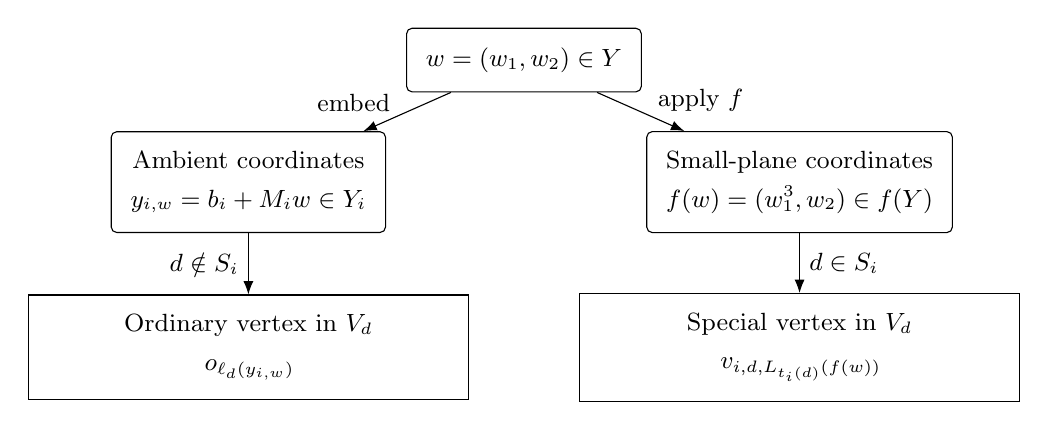
\begin{tikzpicture}[
  >=Latex,
  point/.style={draw,rounded corners=2pt,align=center,inner sep=7pt},
  labelbox/.style={draw,align=center,text width=5.1cm,inner sep=7pt},
  every node/.style={font=\small}]
\node[point] (w) at (0,0) {$w=(w_1,w_2)\in Y$};
\node[point] (old) at (-3.5,-1.55)
  {Ambient coordinates\\[3pt]$y_{i,w}=b_i+M_iw\in Y_i$};
\node[point] (new) at (3.5,-1.55)
  {Small-plane coordinates\\[3pt]$f(w)=(w_1^3,w_2)\in f(Y)$};
\node[labelbox] (ordinary) at (-3.5,-3.65)
  {Ordinary vertex in $V_d$\\[3pt]$o_{\ell_d(y_{i,w})}$};
\node[labelbox] (special) at (3.5,-3.65)
  {Special vertex in $V_d$\\[3pt]$v_{i,d,L_{t_i(d)}(f(w))}$};
\draw[->] (w) -- node[above left,inner sep=2pt,xshift=-4pt,yshift=-2pt] {embed} (old);
\draw[->] (w) -- node[above right,inner sep=2pt,xshift=4pt,yshift=-2pt] {apply $f$} (new);
\draw[->] (old) -- node[left] {$d\notin S_i$} (ordinary);
\draw[->] (new) -- node[right] {$d\in S_i$} (special);
\end{tikzpicture}

\caption{The two label rules for the vertex of \(e_{i,w}\) in part
\(V_d\).  The left branch uses the embedded point \(b_i+M_iw\);
the right branch uses \(f(w)=(w_1^3,w_2)\) in the small plane.
For each \(d\in A_i\), two parameters give the same ordinary label
exactly when their images under \(f\) lie on the same corresponding
horizontal or vertical line.
The diagram records maps and label choices, rather than geometric
positions in the finite plane.}
\label{fig:two-coordinates}
\end{figure}

\begin{proposition}
\label{con-intersection}
The hypergraph \(H\) is intersecting.  Furthermore, all the edges
in its displayed parametrization are distinct.
\end{proposition}

\begin{proof}
There are four types of pairs, according to whether their edges are
ordinary or exceptional and, in the latter case, whether their group
indices agree.

Two ordinary edges with distinct base points share the ordinary
label of their join.  Next, an exceptional base point \(y\in Y_i\)
lies on a deletion line in every direction of the nonempty set
\(S_i\), so \(y\notin X\).  Its join with \(x\in X\) cannot
have direction in \(S_i\): otherwise that join would be a selected
deletion line containing \(x\).  Its ordinary label therefore
belongs to both the exceptional edge and \(e_x\).

For exceptional edges from distinct groups \(i,j\), the base
points are distinct by \eqref{con-separation}.  That same separation
condition ensures that their join has direction outside both
\(D_i\) and \(D_j\), and hence outside \(S_i\cup S_j\).
The two edges share its ordinary label.

Finally, consider \(e_{i,w}\) and \(e_{i,w'}\) with \(w\ne w'\).
The transformed points \(f(w),f(w')\) are distinct.  If their
join has finite nonzero slope \(t\), the exceptional edges share
the special label of this subfield line in the part of direction
\(M_i(t)\).  If their join is horizontal or vertical, the relevant
original coordinates are equal as well, because \(f\) preserves
these two parallel classes bijectively.  The original base points
then share an ordinary axis-direction label, in a direction of
\(A_i\).  This completes the intersection proof.

We also check that the parameters count distinct edges, as required
when we count exceptional edges below.  Two ordinary labels in
nonparallel directions determine the ordinary base point, so ordinary
edges are distinct.
An exceptional edge has special labels and cannot equal an ordinary
edge.  Within one group, the special labels in any two distinct
directions of \(S_i\) determine \(f(w)\), since the corresponding
subfield lines are nonparallel.  As \(|S_i|=s-1\ge2\), equal
exceptional edges within a group would imply \(w=w'\).  Finally,
any special label tagged by group \(i\) is absent from every edge
of a different group.  Exceptional edges in distinct groups are
therefore distinct too.
\end{proof}

\Needspace{14\baselineskip}
\subsection{Covering vertices in the small-plane coordinates}

We identify the positions of the exceptional edges of group \(i\)
with \(f(Y)\), via \(e_{i,w}\leftrightarrow f(w)\).  The action
of a covering vertex means the subset of these positions whose edges
contain that vertex.  The next lemma translates every such action
into one of the two resources in Lemma~\ref{lem:gadget}: a subfield
line or an individual point.

\begin{lemma}
\label{con-label-action}
Fix a group \(i\).
\begin{enumerate}
\item A special vertex of group \(i\) covers the positions on one
subfield line.  A special vertex of another group covers none.
\item An ordinary vertex of direction in \(S_i\) covers none.
An ordinary vertex of direction in \(A_i\), if it covers any
positions, covers them on a single horizontal or vertical line in
the \(f\) coordinates.
\item An ordinary vertex of direction outside \(S_i\cup A_i\)
covers at most one position.
\end{enumerate}
In particular, the positions covered by any one vertex are contained
in a subfield affine line.
\end{lemma}

\begin{proof}
The assertions for special vertices and altered ordinary directions
follow directly from \eqref{con-exceptional-vertex}.  For an axis
direction, undoing \(b_i,M_i\) fixes one original coordinate, so
applying \(f\) gives the corresponding horizontal or vertical
line.  A line in a direction outside \(S_i\cup A_i\) cannot
contain two points of \(P_i\), since the join directions of that
embedded subplane are exactly \(S_i\cup A_i\).  It therefore
covers at most one exceptional position.  A singleton can be
included in an arbitrary subfield line through it, and an empty
set requires no covering resource.
\end{proof}

\subsection{The final cover argument}

\begin{proof}[Completion of the proof of Theorem~\ref{thm:main}]
We prove that \(H\) has no vertex cover of size at most \(q\).
Suppose to the contrary that \(C\) is such a cover.  Its ordinary
vertices, regarded as affine lines, must cover \(X\): special
vertices belong to no ordinary edge.  These lines also cover
\(X_{\rm pool}\).  Lemma~\ref{con-pool-properties} therefore
gives a projective point \(p\) such that at least
\((1-\rho)q\) ordinary vertices of \(C\) are lines through
\(p\).  The line-survival bound will force every undeleted member
of this pencil into \(C\).  We then count the vertices left for
exceptional edges, separating centers at infinity, centers inside one
of the sets \(P_i\), and finite centers outside them all.

\paragraph{Every undeleted line in this pencil is forced.}
We claim that
\begin{equation}
\label{con-forced-pencil}
 p\in\ell,\quad\ell\notin B
 \quad\Longrightarrow\quad o_\ell\in C,
\end{equation}
where incidence with an infinite \(p\) means that \(\ell\) has
the corresponding direction.  If \(o_\ell\) were missing, all
other lines of \(C\) through \(p\) would cover at most one
affine point of \(\ell\).  There are at most \(\rho q\)
vertices outside the large pencil subcollection.  Each of their
ordinary lines covers at most one point of \(\ell\), and their
special vertices cover no ordinary edge.  Consequently
\[
 |X\cap\ell|\le1+\rho q.
\]
This contradicts \eqref{con-selected-line-bound}, since
\(\delta q/2>1+\rho q\) for sufficiently large \(q\) and
\(\rho=\delta/10\).  At infinity the pencil lines are parallel,
so the possible contribution of one central point is absent; the
same upper bound still applies.

Let \(F_p\) be the set of ordinary vertices forced by
\eqref{con-forced-pencil}, and call the vertices of \(C\setminus F_p\)
the additional vertices.  The deleted pencil lines determine how
many additional vertices the assumed budget \(|C|\le q\) permits.

\paragraph{An infinite center.}
Suppose \(p\) is the point at infinity in direction \(d\).  Put
\[
 I_d=\{i\in\mathcal I:d\in S_i\},
 \qquad z=|I_d|\in\{1,2\}.
\]
Only these groups contribute deletion lines in direction \(d\),
and each contributes \(s-1\), by
Lemma~\ref{con-deletion-count}.  At most \(z(s-1)\) of the
\(q\) lines in this parallel class belong to \(B\).  Thus
\[
 |C\setminus F_p|\le z(s-1).
\]
None of the forced vertices covers any exceptional edge of a group
in \(I_d\), because those groups use special vertices in
direction \(d\).

If \(z=1\), all positions of this group's \(f(Y)\) must therefore
be covered by at most \(s-1\) additional vertices.  By
Lemma~\ref{con-label-action}, their effects can be included in at
most \(s-1\) subfield lines.  This contradicts
Lemma~\ref{lem:gadget}.

If \(z=2\), the two groups are \(1,*\), by
\eqref{con-double-directions}.  An additional vertex can now meet
both groups, so we use the weighted line-and-point budget instead of
counting one line per vertex.  For each of these groups let \(a_i\)
count the additional vertices that cover at least one of its
positions and are either special vertices of this group or ordinary
vertices in its axis directions \(A_i\).  Let \(b_i'\) count the
other additional vertices covering a position of the group.  By
Lemma~\ref{con-label-action}, the latter vertices each cover only
a singleton.  The former supply subfield lines.  The weighted
conclusion of Lemma~\ref{lem:gadget} gives
\begin{equation}
\label{con-two-group-lower}
 a_i+\frac{b_i'}2\ge s
 \qquad (i=1,*).
\end{equation}

Each additional vertex contributes at most one to the sum of the
two left sides.  A special vertex is confined to its tagged group.
An ordinary axis-direction vertex counted in \(a_i\) is a line
meeting \(P_i\) with direction in \(A_i\subseteq D_i\); by
\eqref{con-separation} it cannot meet the other group's \(P_j\).
It therefore contributes nothing to that other group, even as a
singleton.  Any vertex of neither exclusive type contributes at
most \(1/2\) to each group.  This accounts for every type of
additional vertex, including those covering neither group.
Summing \eqref{con-two-group-lower}, we obtain
\[
 2s\le a_1+\frac{b_1'}2+a_*+\frac{b_*'}2
 \le |C\setminus F_p|\le2(s-1),
\]
a contradiction.

\paragraph{A finite center inside an embedded configuration.}
Now let \(p\) be finite, and write
\[
 h_p=|\{\ell\in B:p\in\ell\}|.
\]
There are \(q+1\) affine lines through \(p\), so
\begin{equation}
\label{con-finite-budget}
 |F_p|=q+1-h_p,
 \qquad |C\setminus F_p|\le h_p-1.
\end{equation}
The loss of one in the second inequality comes from the \(q+1\)
members of a finite pencil and the assumed cover size \(q\).
If \(h_p=0\), the forced vertices already exceed the permitted
size of \(C\).  We may therefore assume \(h_p\ge1\) in both
finite-center cases.

Suppose \(p\in P_i\), for the necessarily unique such group.
Every deletion line through \(p\) comes from this group: a line
from another group would contradict \eqref{con-separation}, since
its direction belongs to that other group's conflict set.  There
is at most one such line in each direction of \(S_i\), and hence
\begin{equation}
\label{con-internal-pencil-size}
 h_p\le s-1.
\end{equation}
Let \(w_p=M_i^{-1}(p-b_i)\in\F_s^2\), whether or not
\(w_p\in Y\).  We account for the exceptional positions of this
group covered by \(F_p\): they will all lie on two nonparallel
lines in the new coordinates.  For a position with base point
\(y\ne p\), its join with \(p\) has a direction in
\(S_i\cup A_i\).  A direction in \(S_i\) cannot cover this
edge by an ordinary vertex.  Any actual forced coverage must
therefore lie along one of the two axis-direction lines through
\(p\).  A position based at \(p\) itself, if present, lies on
both these axes as well.

Since \(f\) preserves the two coordinate parallel classes, all
these covered positions are contained, in the new coordinates, in
the horizontal and vertical lines through \(f(w_p)\).  The
remaining positions are covered by the additional vertices; each
can be included in one subfield line by
Lemma~\ref{con-label-action}.  Equations
\eqref{con-finite-budget} and \eqref{con-internal-pencil-size}
would thus give a cover of \(f(Y)\) by at most
\[
 2+(h_p-1)\le s
\]
lines containing the two nonparallel coordinate lines. These
are legitimate covering resources whether or not their ordinary labels
belong to \(F_p\): their union contains every position covered by
\(F_p\). Removing any duplicate replacement lines preserves these
two distinct lines and can only decrease the count.  This contradicts
Lemma~\ref{lem:gadget}.

\paragraph{A finite center outside all embedded configurations.}
It remains to consider \(p\notin\bigcup_{i\in\mathcal I}P_i\).
Here we use the five points on each deletion line, rather than the
small-plane cover obstruction.  We will find \(5h_p\) exceptional
edges missed by \(F_p\), while each additional vertex covers at
most five of them.

Each group contributes at most one deletion line through \(p\).
Indeed, two distinct such lines cannot be parallel.  After undoing
\(b_i,M_i\), their subfield affine equations have distinct
subfield directions.  Solving these two equations uses a
nonsingular linear system over \(\F_s\), so their intersection
lies in \(\F_s^2\).  This would place \(p\) in \(P_i\), a
contradiction.  Also, deletion lines from different groups cannot
coincide, by \eqref{con-separation}.

The \(h_p\) deletion lines through \(p\) therefore come from
\(h_p\) distinct groups.  From each such group \(i\), choose five
distinct points of \(Y_i\) on its contributing line, possible by
Lemma~\ref{con-deletion-count}.  These give \(5h_p\) distinct
exceptional edges, by Proposition~\ref{con-intersection}.  None
is covered by a forced ordinary vertex: its unique join line to
\(p\) is precisely its contributing deletion line, whose
direction is altered for that group.

Any one additional vertex covers at most five of these selected
edges.  For a special vertex this follows because it belongs to
only one group.  An ordinary line through \(p\) covers none,
by the same unique-join and altered-direction argument.  Finally,
let an ordinary vertex \(o_\ell\), with \(\ell\) not through
\(p\), cover some selected edges.  The line \(\ell\) meets each
contributing line in at most one point, so \(o_\ell\) covers at most
one selected edge from each contributing group.  Every such group
has a selected point \(y\in Y_i\cap\ell\) whose join to \(p\)
has direction in \(S_i\).  The third part of
Lemma~\ref{con-pool-properties}, which applies to all candidates
and hence to the selection, bounds the number of these groups by
five.  This proves the asserted bound for every additional vertex.

By \eqref{con-finite-budget}, at most \(h_p-1\) additional
vertices are available.  They can cover at most \(5(h_p-1)\) of
the \(5h_p\) selected edges, a final contradiction.

We have ruled out every possible projective center \(p\), and
hence every vertex cover of size at most \(q\).  Therefore
\(\tau(H)\ge q+1\).  Conversely, any edge of the nonempty
intersecting hypergraph \(H\) is itself a vertex cover and has
size \(q+1\).  It follows that
\[
 \tau(H)=q+1.
\]
The parameter choices in Section~\ref{sec:placement} give this
hypergraph for every sufficiently large odd integer \(n\), with
\(q=s^n\), after fixing any sufficiently large prime
\(s\equiv2\pmod3\) and a successful \(Y\). Choose one such \(Y\)
for each eligible \(s\), and let \(n_0(s)\ge3\) exceed all the
resulting degree thresholds. This proves Theorem~\ref{thm:main}.
Since there are arbitrarily large odd integers, it also gives infinitely
many ranks \(r=q+1\).
\end{proof}


\Needspace{32\baselineskip}
\bibliographystyle{plain}
\bibliography{references}
\end{document}
